\chapter{Computational Modelling of Tissue Ablation}
\label{chap:ablation}
\section{Introduction and Background}
\label{sec:intro}

This chapter uses \gls*{mcrt} techniques coupled to a heat transfer simulation, to study the thermal damage to tissue due to a laser, with its power spread over many beams to leave viable tissue around zones of damaged/necrotic tissue~\cite{manstein2004fractional}. This class of laser is called a fractionated ablative laser. This chapter presents experimental work carried out on porcine tissue by our collaborators at the University of Dundee and the photobiology department at Ninewells Hospital, alongside my computational model of tissue ablation.

\medskip

Ablative lasers are used in a wide variety of medical procedures including: coagulating scalpels, port wine stain removal, tattoo removal, hair removal, and skin rejuvenation~\cite{amini2010ultrafast, tan1989treatment,kuperman2001laser,liew2002laser,hardaway2002nonablative}.
One class of laser used in these procedures are ablative lasers. Ablative lasers are usually high powered lasers ($>$30~W) targeted at a specific chromophore in the skin, to partially or fully remove layers of skin. These types of lasers are commonly used for aesthetic procedures such as: skin rejuvenation~\cite{hardaway2002nonablative}, and removal of various diseases such as Rhinophyma~\cite{shapshay1980removal} or lesions/nodules~\cite{valcavi2010percutaneous}. Ablative lasers have also been recently investigated as a means of better drug penetration into the skin for various therapies such as \gls*{pdt}. The ablative laser ``drills'' holes in the skin, which allows topical treatments to better diffuse into the skin~\cite{haedersdal2010fractional}.

One downside to using lasers to remove tissue, is that unlike a scalpel where the surgeon has full control of the depth of the incision, ablative lasers are not as predictable. Lasers can cause thermal damage to the surrounding areas, leading to potentially  unwanted effects, though some applications of ablative lasers utilise the thermal damage, particularly aesthetic procedures~\cite{alexiades2008spectrum}.

Currently, the standard method to measure the depth of the ablative holes is via a biopsy which is an invasive procedure. In this work an \gls*{oct} system is used to measure the ablative crater non-invasively \textit{in-vivo}. The \gls*{oct} measurements are then compared to a computational model developed as part of this project. It is hoped this computational model could be used to predict the depth of the ablative crater when using a certain laser power for various different applications such as: laser assisted drug delivery, and various cosmetic applications.


\section{Methods}

To replicate the experimental work \textit{in silico}, the numerical model has three main portions. The first is the \gls*{mcrt} code that models light transport through tissue so that we can calculate the laser energy deposited as a function of time and space. The second, a \gls*{fdm} which is used to calculate the heat diffusion within the tissue due to the absorbed laser energy. Finally, a tissue damage model to track the tissue damage caused by the laser. All these individual functions are connected together to create a full numerical model.
The full code from this chapter can be found at \url{https://github.com/lewisfish/Tissue-Ablation-MC}

\subsection{Monte Carlo radiation transport (MCRT)}

\gls*{mcrt} is used here to calculate the energy deposited by the laser. This is then passed to the heat transport simulation, which calculates the heat diffusion in the medium. The algorithm for the three coupled simulations is presented in~\cref{fig:algoablation}.

\begin{figure}[!htbp]
\centering
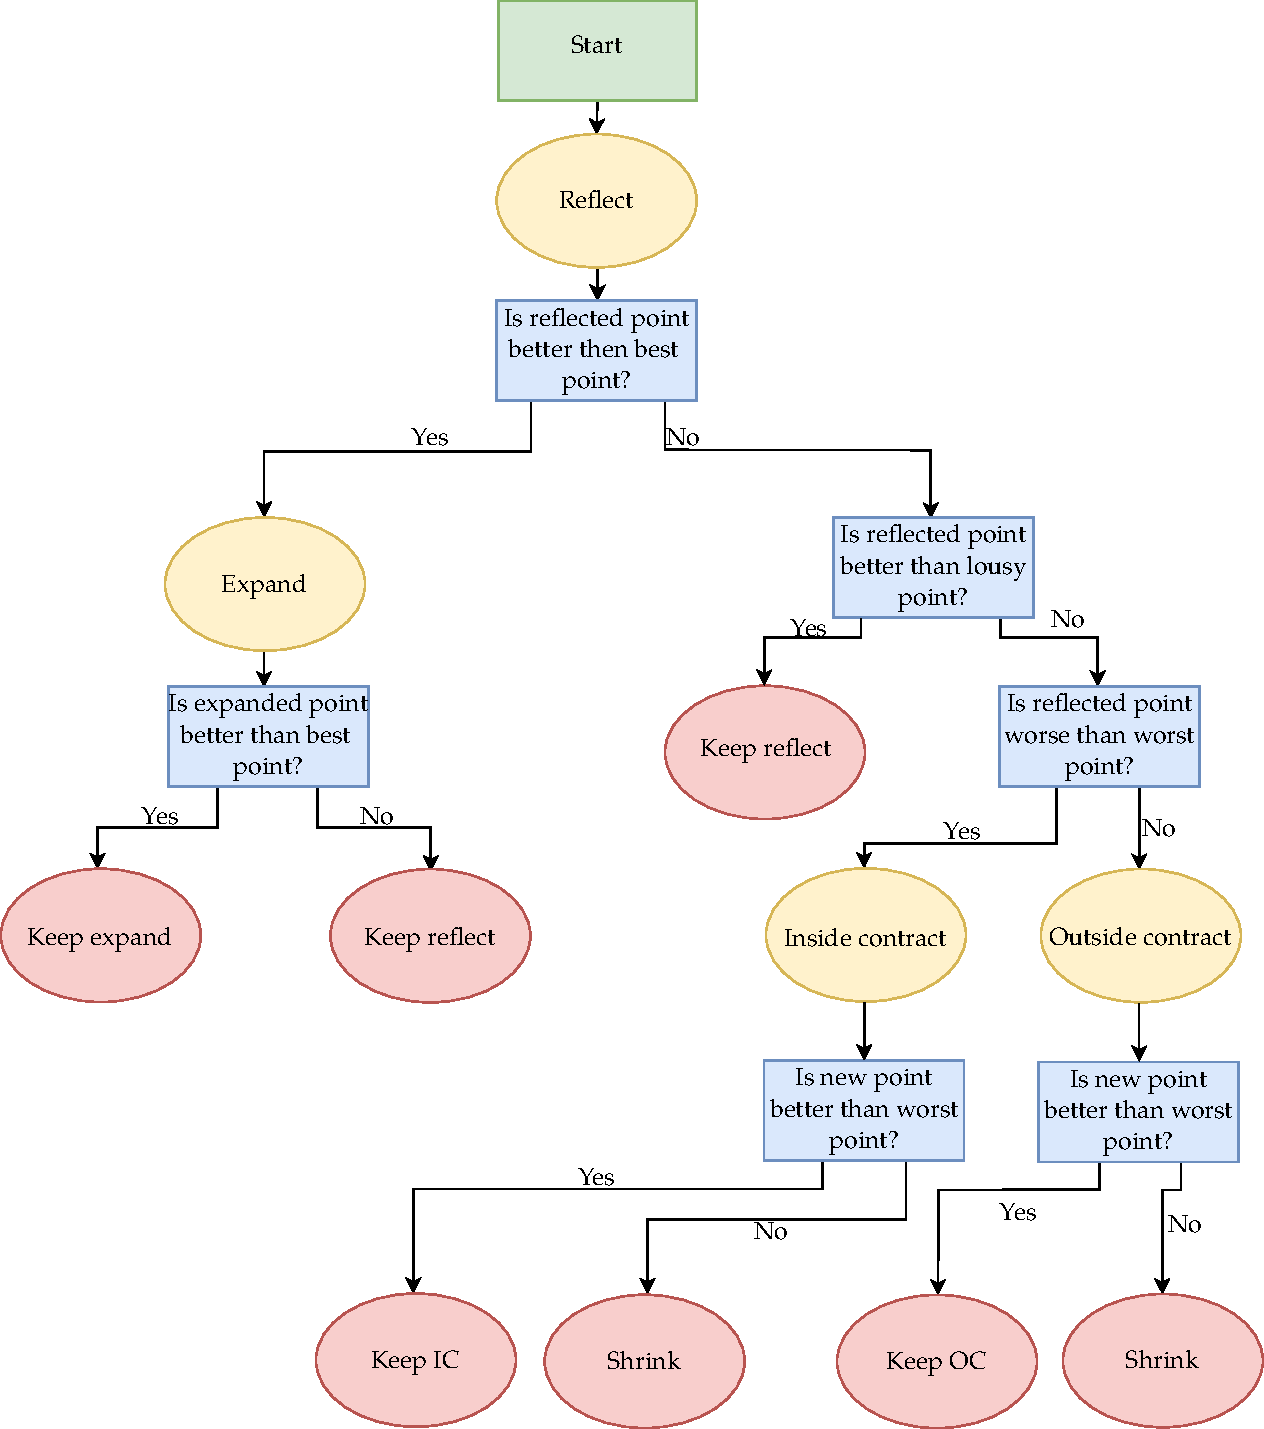
\includegraphics[scale=0.7]{flowchart.pdf}
\caption{Flowchart of the tissue ablation algorithm.}
\label{fig:algoablation}
\end{figure}

The \gls*{mcrt} algorithm is largely the same as described in~\cref{sec:mcrt}, with some important adjustments.

The first adjustment is that the path length counter for fluence is changed to track absorbed energy. This is achieved by multiplying the pathlength in a voxel by the absorption coefficient of that voxel. \Cref{fig:jmea-explain} show this process graphically, and \Cref{eqn:ablationenergy} shows the mathematical expression:

\begin{equation}
E_{i}^{abs} = \frac{P}{N V_i}\sum\mu_{a,i} s
\label{eqn:Eabs}
\end{equation}

\noindent Where:

	\indent $E_i^{abs}$ is the energy absorbed in the $i^{th}$ voxel [$Js^{-1}m^{-3}$];
	
	\indent $P$ is power [$W$];
	
	\indent $N$ is the number of packets, representing a power, $P_i$;
	
	\indent $V_i$ is the volume of the $i^{th}$ voxel [$m^{-3}$];
	
	\indent $\mu_{a,i}$ is the absorption coefficient of the $i^{th}$ voxel [$cm^{-1}$];
	
	\indent and s is the pathlength of a packet through the $i^{th}$ voxel [$cm$].
	
	\medskip
	
\begin{figure}[!htbp]
\centering
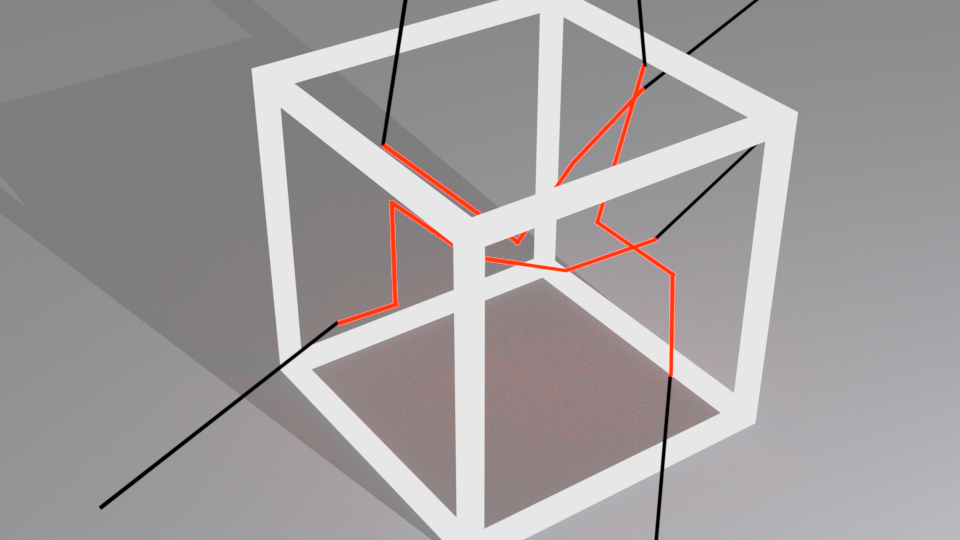
\includegraphics[scale=0.25]{jmea-explain.png}
\caption{Red lines are packet paths within a voxel. Black lines packet paths out with the voxel. Red packet paths, weighted by $\mu_a$, are summed up to calculate the absorbed energy within each voxel.}
\label{fig:jmea-explain}
\end{figure}	
		
This grid of absorbed energy is then passed to the heat transport portion of the simulation, so that the heat diffusion in the porcine tissue can be calculated.

The next adjustment to the \gls*{mcrt} algorithm is that the \gls*{mcrt} algorithm is run for every heat simulation time step, as the medium could change at every time step due to the optical, and thermal properties changing as a function of tissue damage.

Finally, to match the experiment undertaken the medium and laser for the \textit{in-silico} experiments must match the practical experiments. As the laser used in the experiments emits an infra-red wavelength ($10.6~\mu m$), the optical properties are dominated by the water content of the tissue. Due to this it is assumed that there is just absorption in the medium, with no scattering. Further discussion can be found in~\cref{sec:opticalprops}. The laser in some of the \textit{in silico} modelling, has multiple beams and the source photon packet routine is adjusted to accommodate this when needed.

\subsection{Heat Transport}

The diffusion of heat can be modelled using the heat equation~(\cref{eqn:heat}), which is derived from Fourier's law and the principle of conservation of energy~\cite{widder1976heat}.  The standard heat equation is a partial differential equation of the parabolic form. Solutions and analytical methods are readily available for lower dimensions (i.e. 1D heat diffusion), but for higher dimensions, numerical models must be used for all except the simplest problems. The simplest form of the heat equation is shown below:

\begin{equation}
\rho c_p \frac{\partial T}{\partial t}= \nabla \cdot (\kappa \nabla T) + \dot{q}
\label{eqn:heat}
\end{equation}

\noindent Where:

	\indent $T(x, y, z, t)$ is the temperature as a function of time and space [\textit{K}];
	
	\indent $\kappa$ is the thermal conductivity [$W m^{-1} K^{-1}$];
	
	\indent $\rho$ is the density [$kg  m^{-3}$];
	
	\indent $c_p$ the specific heat capacity [$J K^{-1}$];
	
	\indent $\dot{q}(x,y,z,t)$ is the source/sink term as a function of time and space [$W m^{-3}$].
	
	\medskip

\Cref{eqn:heat} is for a homogeneous system where the thermal properties do not change as a function of time, space and temperature. However, to model a moving ablation front the nonlinear heat equation must be used, where the thermal properties can be a function of time, space and temperature~(\cref{eqn:nonlinearheat}).

\begin{equation}
\frac{\partial T}{\partial t} = \frac{1}{(\rho c_p)_{\xi}}(\nabla k_\xi T + k_\xi\nabla^2T)+\dot{q},\quad \text{where}\ \xi=(i,j,k)
\label{eqn:nonlinearheat}
\end{equation}

Included in~\cref{eqn:nonlinearheat} is a source and sink term, $\dot{q}$, to allow the modelling of heat loss/gain from external sources/sinks. The heat source in this simulation is due to the laser, and it is assumed that the only loss of heat to the surrounding medium is via conduction.
	
The medium is considered to be at a constant temperature of 5$^{\circ}$C, as the porcine skin was kept cooled prior to experimental work and the simulation volume is smaller than the porcine tissue samples. 
%The face of the medium on which the laser is incident, has a simple convective BC (based upon Newton's law of cooling):	

% \begin{equation}
% \dot{q}_c = -hA(T - T_\infty)
% \label{eqn:bceqns}
% \end{equation}

% \noindent Where:

% 	\indent \textit{h} is the heat transfer coefficient [$W m^{-2} K$];
	
% 	\indent \textit{A} is the area of the grid element, that is radiating/convicting heat away [$m^{-2}$];
	
% 	\indent and $T$, and $T_\infty$ are the temperature in a voxel and the surrounding medium temperature respectively~[$K$].
	
% 	\medskip

As \cref{eqn:nonlinearheat} is generally hard to solve in arbitrary geometries with complex boundary conditions, a numerical method is employed to solve it.
The numerical method employed is a finite difference method (FDM), derived from the Taylor series, see~\cref{eqn:taylor}. 


The \gls*{fdm} works by discretising a function, $f(x)$, onto a grid with \textit{N} nodes a distance $\Delta x$ apart. ~\Cref{eqn:taylor} is then truncated and rearranged and it is assumed that the remainder term $R_1$ is sufficiently small enough, to yield an approximation for the first derivative of a function $f(x)$ at a point $x_0+\Delta x$, see~\cref{eqn:fdmfirst}.
\Cref{eqn:fdmfirst} is the so called ``forward'' difference, due to it using a point in the ``forward'' direction.
The ``backward'' and ``central'' difference terms can be calculated by using a node at $x_0-\Delta x$ for the backward difference~\cref{eqn:fdmbck}.
The central difference (~\cref{eqn:fdmcent}) is an average of the forward and backward differences.
Expressions can also be given for the $2^{nd}$ derivatives for backward, forward and central (forward and backward $2^{nd}$ order equations omitted for brevity)~\cref{eqn:fdmcent2}.

\begin{equation}
f(x_0+\Delta x)=f(x_0) + \frac{f'(x_0)}{1!}\Delta x + \frac{f''(x_0)}{2!}\Delta x^2+...+ \frac{f^{(n)}(x_0)}{n!}\Delta x^n+R_n(x)
\label{eqn:taylor}
\end{equation}

\begin{equation}
f'(x_0) \approx \frac{f(x_0+\Delta x)-f(x_0)}{\Delta x}
\label{eqn:fdmfirst}
\end{equation}

% \begin{figure}
%   \begin{center}
%     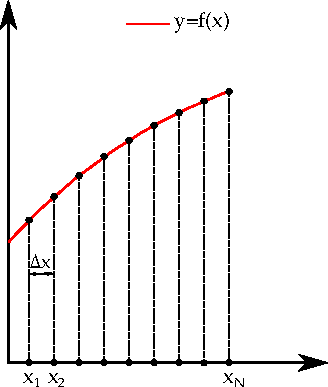
\includegraphics[width=0.48\textwidth]{fdm.pdf}
%   \end{center}
%   \caption{Discretisation of \text{f(x).}}\label{fig:fdmexplain}

% \end{figure}

\begin{subequations}
\begin{align}
\frac{df}{dx} &= \frac{f_{i+1} - f_{i}}{\Delta x}\footnotemark  &(forward) \label{eqn:fdmfwd}\\
\frac{df}{dx} &= \frac{f_{i} - f_{i-1}}{\Delta x}  &(backward) \label{eqn:fdmbck}\\
\frac{df}{dx} &= \frac{f_{i+1} - f_{i-1}}{2\Delta x}  &(central)\label{eqn:fdmcent}\\
\frac{d^2f}{dx^2} &= \frac{f_{i-1}-2f_i+f_{i+1}}{\Delta x^2} &(central)\label{eqn:fdmcent2}
\end{align}
\end{subequations}
\footnotetext{For brevity $f(x_0+\Delta x)$ is defined as $f_{i+1}$, and $f(x_0-\Delta x)$ as $f_{i-1}$, etc.}

Thus, the linear heat equation~\cref{eqn:heat}, in 1D, taking a $1^{st}$ order forward time derivative, and a $2^{nd}$ order central spatial derivative gives:

\begin{subequations}
\begin{align}
\frac{T^{n+1}_i-T^{n}_i}{\Delta t} &= \alpha\frac{T^n_{i-1}-T^n_{i}+T^n_{i+1}}{\Delta x^2}  + \frac{\dot{q}}{\rho c_p}\\
T_{i}^{n+1} &=  \alpha\Delta t \frac{T_{i-1}^n-2T_i^n+T_{i+1}^n}{\Delta x^2} + \frac{\Delta t\dot{q}}{\rho c_p}
\label{eqn:simplefdm}
\end{align}
\end{subequations}

Where $\alpha=\tfrac{\kappa}{\rho c}$.

\begin{figure}
  \begin{center}
    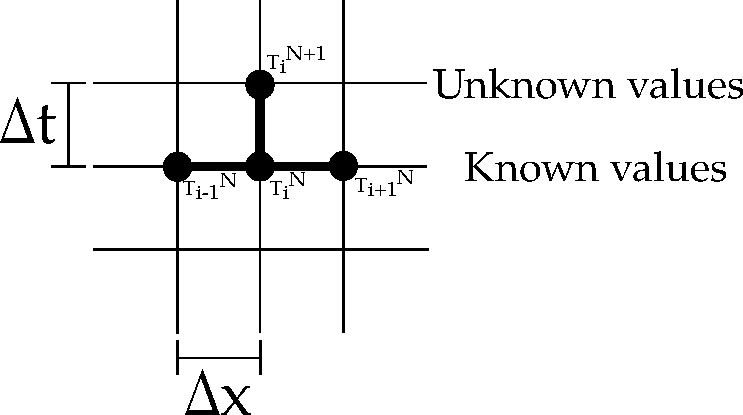
\includegraphics[width=0.48\textwidth]{fdm-stencil.pdf}
  \end{center}
  \caption{Finite difference method stencil for simple explicit scheme.}
  \label{fig:fdmstencil}
\end{figure}

\Cref{eqn:simplefdm} is called the ``simple explicit form of finite-difference approximation''\cite{ozisik1994finite}. \Cref{fig:fdmstencil} shows the ``stencil'' of this scheme, where there are three known points at time \textit{N}, and just one unknown at time \textit{N+1}. There are various other schemes that can be used to calculate the temperature at the next time step. However, the simple explicit scheme is used here due to its ease of implementation despite there being a constraint on the time step used in comparison to an implicit method where there is none. This method is also easily scaled up to 3D with little difficulty.

\medskip

For the more complicated nonlinear heat equation there is a possibility that the medium is not continuously smooth between nodes, in terms of optical and thermal properties. The two easiest methods~\cite{ozisik1994finite} of achieving this are: (1), lag the value behind by one step, i.e $c_{p}^{n+1}=c_{p}^{n}$. (2), average $\kappa,\ \rho,\ \text{and}\ c_p$ using a half difference scheme where the thermal property used in the calculation is the thermal property halfway between two nodes, i.e the average of the two nodes:

\begin{align}
\kappa^{\pm}&=\frac{\kappa_i+\kappa_{i\pm 1}}{2}\\
\rho^{\pm}&=\frac{\rho_i+\rho_{i\pm 1}}{2}\\
c_p^{\pm}&=\frac{c_{p,i}+c_{p,i\pm 1}}{2}
\end{align}

Thus, for the simple 1D case as in~\cref{eqn:simplefdm}, the thermal properties are averaged between nodes when computing the coefficients of the temperature nodes, and lag the thermal properties when adding the heat from the laser:

\begin{equation}
T^{N+1}=\Delta t (AT^N_{i-1}-2BT^N_{i}+DT^N_{i+1})+ T_i^N + \frac{\Delta t\ \dot{q_L}}{\rho c_p}\label{eqn:heatnonlin1d}
\end{equation}

Where (in the $x$ direction):
\begin{align}
A=&\frac{\kappa^{-}}{\rho^{-}c_{p}^{-}2\Delta x^2} \nonumber \\
B=&\frac{\kappa^{+}}{\rho^{+}c_{p}^{+}2\Delta x^2} \label{eqn:coeffsABD}\\
D=&\frac{(A+B)}{2} \nonumber
\end{align}

\Cref{eqn:heatnonlin1d} is straightforward to generalise to higher dimensions. The 3D case gives:

\begin{align}
U_{xx} &=  (A T^N_{i-1,j,k} - 2B T^N_{i,j,k} + D T^N_{i+1,j,k}) \label{eqn:FDMheat1}\\
U_{yy} &=  (A T^N_{i,j-1,k} - 2B T^N_{i,j,k} + D T^N_{i,j+1,k}) \label{eqn:FDMheat2}\\
U_{zz} &=  (A T^N_{i,j,k-1} - 2B T^N_{i,j,k} + D T^N_{i,j,k+1}) \label{eqn:FDMheat3}\\
T^{N+1}_{i,j,k} &= \Delta t\ (U_{xx} + U_{yy} + U_{zz}) + T^{N}_{i,j,k} + \tfrac{\Delta t}{\rho c_p}\dot{q_L} \label{eqn:FDMheat4}
\end{align}

\noindent Where:

	\indent $T^{N+1}_{i,j,k}$ is the new temperature at node $i,j,k$ [$K$];
	
	\indent $T^N_{i,j,k}$ is the temperature at node $i,j,k$ at the current time step [$K$];
	
	\indent $\alpha$ is the thermal diffusivity [$m^2 s^{-1}$];
	
	\indent $\kappa$ is the thermal conductivity [$W/m K$];
	
	\indent $\Delta x\ etc.$ is the size of the grid element in the $p^{th}$ direction [$m$];
	
	\indent and $A, B,D$ are the coefficients in their respective dimension (\cref{eqn:coeffsABD}).

	\medskip
	
\Cref{eqn:FDMheat4} gives the full numerical solution to the nonlinear heat equation with a laser heat source. This will allow the calculation of the heat diffusion in the porcine tissue due to laser heating.

\medskip

As the laser used in the experimental work operates in a pulsed mode, this is accounted for in the simulation. The laser pulse shape is a triangular pulse, with the peak power, $P_{peak}$, and pulse length, $\tau$~\cite{pixelco2manual}. In the heat simulation there has to be an additional variable in the term $laserOn(t)\cdot\tfrac{\alpha \Delta t}{\kappa}\dot{q_L}$ in \cref{eqn:FDMheat4}. This additional variable, $laserOn(t)$, is a boolean value and a function of time, which is defined as:

\[   
laserOn = 
     \begin{cases}
       \text{1,} &\quad\text{Laser on}\\
       \text{0,} &\quad\text{Laser off}.\\
     \end{cases}
\]

In the instance where there is a train of laser pulses, the laser is turned on and off based upon the pulse frequency.

\medskip

Due to a simple explicit \gls*{fdm} being used, the time step is constrained to make the solution stable. For a cubic 3D \gls*{fdm} without prescribed flux boundary conditions, this yields the constraint: $\Delta t \leq \tfrac{1}{\delta \alpha}$ where $\delta=\tfrac{1}{\Delta x^2}+\tfrac{1}{\Delta y^2}+\tfrac{1}{\Delta z^2}$. Along with this time constraint, the pulse length of the laser also has to be considered. If the time step of the heat simulation is too large it will not account for the heat deposited by the laser. Thus, the timestep has to be at least an order of magnitude smaller than the shortest laser pulse.

As the time step is small, and the grid resolution large the resultant simulation is slow. Thus, the code has been fully parallelised to improve performance. Both the \gls*{mcrt} and heat simulation are independently parallelised. 

\medskip

Parallelisation of the heat simulation is more involved than the ``embarrassingly parallel'' class of problems where \gls*{mcrt} belongs. This is due to the heat simulation being dependent on neighbouring nodes to update the temperature at the current node. Thus, if the medium were to be split up on to separate cores, there would have to be communication between the cores, in order for the simulation to be completed successfully. Therefore it is not possible to take the ``easy'' route of running the simulation concurrently $N$ times and collating the result at the end of all the simulations.


\begin{figure}[!htbp]
\squeezeup{5.5}
\centering
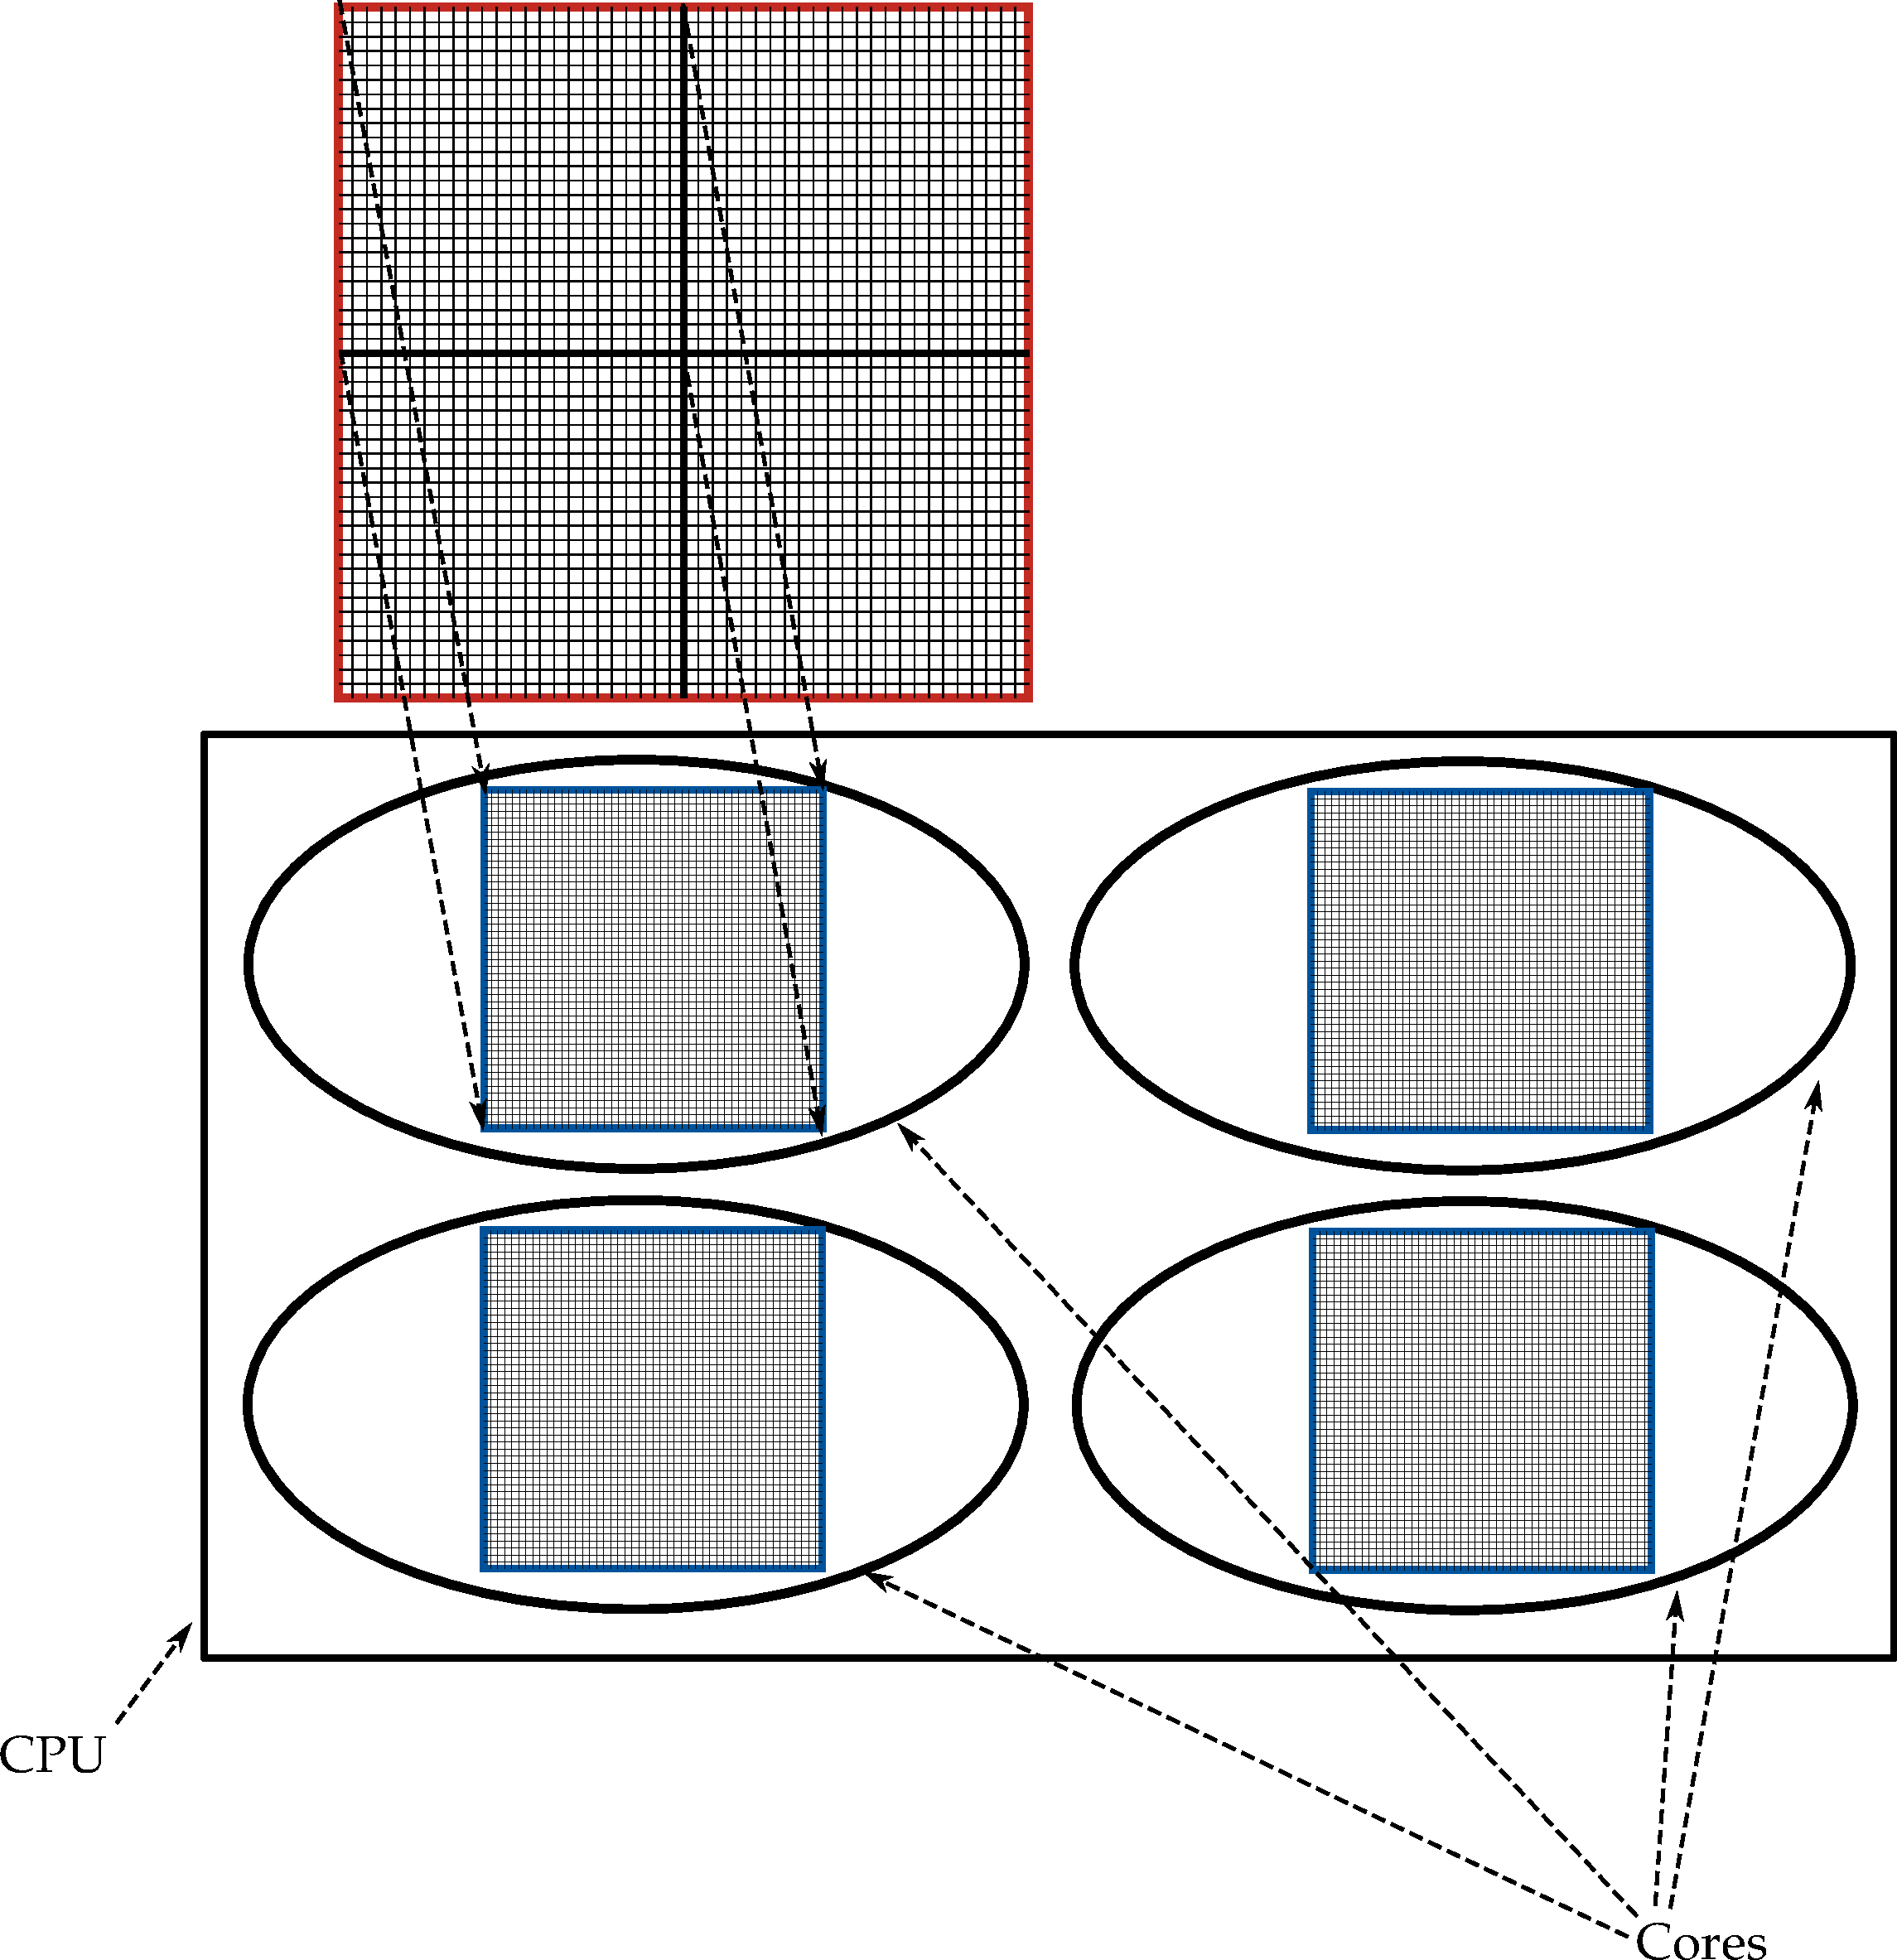
\includegraphics[width=0.75\textwidth]{grid-decomp.pdf}
\caption{Computational domain decomposition. Total computational domain (red outline) is evenly divided between cores in the CPU. This is done via layers of the domain in the z direction. Information is passed to/from cores via the ``halo swap'' process (see~\cref{fig:haloswap}).}
\label{fig:griddecomp}
\squeezeup{5.5}
\end{figure}

The heat simulation is parallelised using a technique called ``halo swapping''. This involves splitting up the computational domain (see \cref{fig:griddecomp}), in this case the tissue medium, and doing the calculations on each domain on a separate core. The ``halo swapping'' comes in when cores need to communicate with each other about updating their boundary temperature nodes (see \cref{fig:haloswap}).

\Cref{fig:parallel} shows the speed up gained from using the technique. The ``halo swapping'' technique is efficient for situations where the computational domain can be split up with large ``chunks'' being calculated on each core. However, if the computational domain is small, and the number of cores large then bottlenecks occur due to too much communication between cores taking place. Thus, to efficiently use ``halo swapping'' careful thought has to be given to the size of the computational domain, and the number of cores running the simulation. Evidence of this bottlenecking can be seen in~\cref{fig:parallel} for problems where the size of the grid, in voxels, is $40^3$ and $24^3$. These problems also show superlinear speed up, for a certain number of cores. This is not unfeasible, due to several reasons, including the start up time of MPI or the underlying computer architecture~\cite{ristov2016superlinear}.

%Use more on amadahls law
%led to a speed up of $\sim$6, over the serial simulation. Using Amdahl's law\cite{amdahl1967validity}, the serial portion of the simulation is $\sim$ 5\%, giving a theoretical speed up $\sim$ 20 times the serial simulation.

\begin{figure}[!htbp]
\squeezeup{3.5}
\centering
\def\svgwidth{250pt}
\input{./ablation/images/halo.pdf_tex}
\caption{Halo swapping. Process A updates the area in red and blue on the left. It updates the blue area which is sent to process B as B's ``halo''. Process B cannot update its own halo, but rather updates the halo for process A.}
\label{fig:haloswap}
\squeezeup{4.5}
\end{figure}

\begin{figure}[!htbp]
\centering
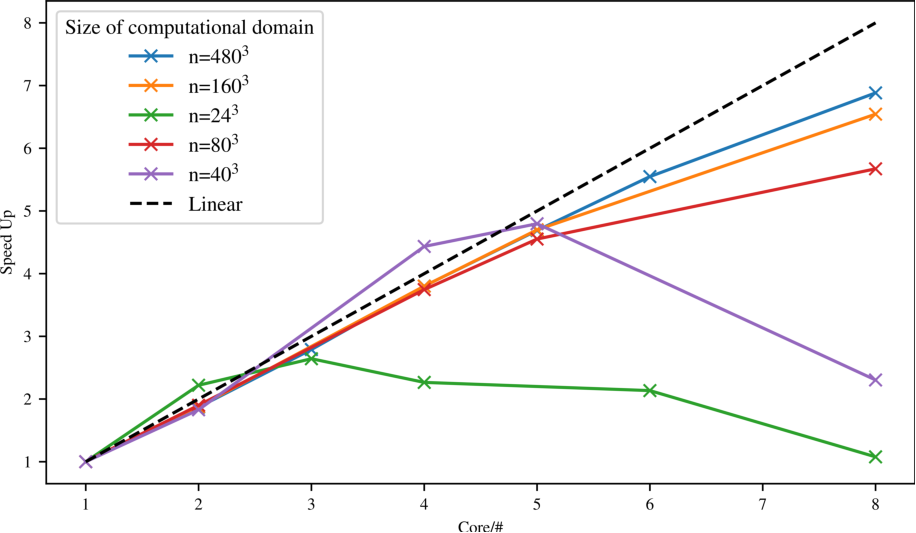
\includegraphics[scale=.55]{profile.pdf}
\caption{Figure shows the speed up gained by parallelisation of the heat simulation using the ``halo swapping'' technique, for various sizes of computational domain (voxels). Data taken from a Intel Xeon E3--1245 v5, 8 cores @ 3.5GHz machine.}
\label{fig:parallel}
\end{figure}

After one time step of the heat simulation has been completed, the temperature grid is passed to the tissue damage portion of the simulation to calculate the tissue damage that may have accrued during the heat simulation time step.
\FloatBarrier

\subsection{Tissue Damage}
\label{sec:tissuedamage}

\subsubsection*{Introduction}
The final portion of the simulation is the tissue damage model.
To be able to model the tissue damage process, the physical reality of this process must be understood.
When the laser is turned on, the temperature starts to rise within the tissue due to the absorption of photons by the tissue. The temperature rise causes damage to the tissue when above a threshold temperature, $T_d$, approximately 43$^{\circ}C$~\cite{welch2011optical}.
From the temperature, $T_d$, four main areas of tissue damage are defined:


\begin{equation}
T = 
     \begin{cases}
       \text{coagulation,} &\quad T_d\leq T \leq 100~^{\circ}C\\
       \text{water boils,} &\quad T=100~^{\circ}C\\
       \text{carbonisation,} &\quad 100~^{\circ}C \leq T \leq T_a\\
       \text{ablation,} &\quad T=T_a.\\
     \end{cases}
\end{equation}


The area of tissue damage termed ``coagulation'' is a multifaceted process. At 43$^{\circ}$C - 50$^{\circ}$C, bonds break within cell membranes, causing ruptures and some cell death~\cite{welch2011optical,wright2015quantitative}. This process is usually termed \textit{hyperthermia}. Around 50$^{\circ}$C, enzyme activity decreases, cells become immobile, and various cell repair mechanisms are disabled, leading to increased cell death. When temperatures exceed 60$^{\circ}$C, proteins become denatured. Thermal denaturation is a structural and functional change in a protein due to the heating it undergoes. This means they change from a highly organised structure with specific purposes, to disorganised structures with little to no function at all~\cite{niemz2013laser}.  %A classic example of denaturation of proteins, is in cooking eggs. Denaturation occurs when the clear fluid egg white, rich in protein albumin, becomes a solid white~.

The next stage in the tissue damage process is the vaporisation of water. As the temperature of the tissue starts to approach 100${^{\circ}}$C (at 1 atm), water starts to vaporise. If the vaporised water cannot escape the tissue it forms steam vacuoles, small pockets of steam. These vacuoles can easily been seen when viewing tissue samples after tissue has been treated with a high powered laser (see \cref{fig:histology}). In certain conditions these steam pockets can explode~\cite{petrella2013popcorn}.


The third stage of tissue damage is carbonisation of the tissue. This occurs when most of the water has boiled off, leaving the remaining tissue to heat up and reduce to its elemental carbon form. This carbonisation of tissue, when it occurs, is generally only a thin layer of 5-20~$\mu m$~\cite{welch2011optical,verdaasdonk1990explosive}.

The final stage of tissue damage is the removal of the remaining tissue, i.e tissue ablation. There is no agreement in the literature how tissue undergoes ablation with several methods proposed. The three main methods are: photochemical, thermal, and explosive~\cite{husinsky1990mechanisms,kitai1991physics,oraevsky1991pulsed}. 
Photochemical ablation is when the energy of a photon from the irradiating laser, is sufficient enough that it excites the electronic state of the tissues molecules into an anti-boding state, leading to broken bonds and conversion from electronic energy into kinetic energy, and thus ablation.
Thermal ablation is where tissue is heated sufficiently so that tissue vaporisation takes place. 
Finally, explosive ablation is an extreme version of thermal ablation. Explosive ablation occurs when large amounts of energy is deposited in a small time scale, so that none of the energy can thermally diffuse away, resulting in explosive ablation.
Photochemical ablation, is usually applied to UV laser ablation, whereas thermal and explosive ablation regimes are the more likely candidates for IR ablation which is considered here.

The theoretical models behind explosive and thermal ablation models are also not well understood, with many models proposed to try and explain experimental results. These models range from heuristic models to sophisticated models that relate the underlying physical mechanisms to ablation damage. 
The two main heuristic models are: the blow off model, and the steady state model. 
The blow off model assumes that there is thermal confinement (i.e no propagation of heat in time $t$), and that material is removed after the laser irradiation. There is a radiant threshold that has to be met to ablate material, and that Beer-Lambert's law describes the spatial distribution of light. For laser pulses of $<10$~ns, these conditions are normally met. However, for lasers with pulse length larger than this, these conditions are not usually met~\cite{vogel2003mechanisms,koren1984emission,andrew1983direct}. 

The steady state heuristic model, assumes that the pulse length is of the order of $ms$ or larger, that material starts to be removed shortly after laser irradiation begins, and that some radiant threshold exists in order for ablation to begin. The steady state model also assumes that a fixed energy is required to remove a unit of tissue~\cite{vogel2003mechanisms}. However, this does not always hold, as there are many circumstances where there is no one fixed energy, but rather many energies (due to various phase changes) that must be met in order for ablation to occur. There are also many other sophisticated models that try to describe what happens physically when ablation occurs~\cite{mckenzie1990physics,mckenzie1986three,majaron1999thermo}.

Due to the above mentioned reasons, there is no defined ablation temperature. The literature, however, does suggest that it takes place when the tissue temperature is between 177~${^{\circ}}$C and 500~${^{\circ}}$C~\cite{gerstmann1994char,mckenzie1986three,sagi1992heating}. 

\begin{figure}	
\vspace{-10pt}
	\centering
	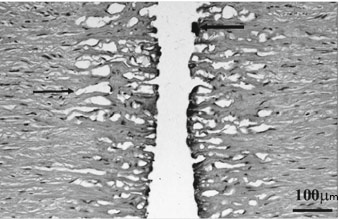
\includegraphics[width=.5\textwidth]{steam_vacoule.png}
	\caption{Ablation of a dog aorta, as viewed under a microscope. Steam vacuoles are clearly visible on either side of the ablation area. Carbonisation is also evident at the edges of the ablation fronts. Adapted from~\cite{welch2011optical}.}
	\label{fig:histology}
	\vspace{-10pt}
\end{figure}

To model all these tissue damage processes the tissue damage model is split into two sections: coagulation damage and ``physical'' damage. Coagulation damage has no effect on the tissue's bulk optical or thermal properties. ``Physical'' damage changes the tissue optical and thermal properties.

\subsubsection*{Modelling coagulation damage}\label{sec:coagdamage}
With the description of the various processes that tissue undergoes during ablation, a numerical model of these processes can be created.
First to model the full extent of the damage done under 100${^{\circ}}$C, i.e in the coagulation regime, the Arrhenius damage model is used. The Arrhenius damage model was originally used as a kinetic model of reaction products in chemistry~\cite{pearce2009relationship}. It has since been adapted by various authors for modelling tissue damage, and is the \textit{de facto} standard~\cite{hendriques1947studies,jiang2002effects}. These authors and various others, adapted this model by fitting~\cref{eqn:arrhenius} to experimental data for burn damage. The two parameters fitted are A, the frequency factor, and $\Delta E$, the activation energy.

\begin{equation}
\Omega(t)=\int^{t_{f}}_{t_i} Ae^{(-\tfrac{\Delta E}{RT})}d\tau
\label{eqn:arrhenius}
\end{equation}


\noindent Where:

	\indent $\Omega$ is the damage value [-];
	
	\indent A is ``frequency factor'' [$s^{-1}$];
	
	\indent $\Delta E$ is activation energy [$J mol^{-1}$];
	
	\indent R is the universal gas constant [$J mol^{-1} K^{-1}$];
	
	\indent T is the temperature [$K$];
	
	\indent and $t_i$ and $t_f$ are the initial time and final time at $t_{crit}$.
	
	\medskip

It is reported that a value of $\Omega$ of 0.53, 1.0, and 10$^4$ relate to first, second, and third degree burns respectively~\cite{diller1983finite}. The Arrhenius damage model is used to better understand the amount of damage caused by the laser in the non-ablated areas of tissue. Values of $A=3.1\times10^{98}$ and $\Delta E=6.3\times10^5$ are adopted~\cite{zhang2007dynamic,sagi1992heating,hendriques1947studies}.

\subsubsection*{Modelling physical tissue damage}

As tissue mostly consists of water~\cite{meglinski2002quantitative} when the temperature of the tissue approaches 100$^{\circ}$C (at 1 atm), water in the tissue begins to boil off. This acts as a large heat sink for the absorbed laser energy, slowing down the rate of ablation. The energy required to boil the water is $Q_{vapor}=m_v\cdot L_v$, where $m_v$ is the mass of a voxel, and $L_v$ is the latent heat of vaporisation. The energy to boil off the water is provided via the laser and heat diffusing into the voxel:

\begin{equation}
Q_{vapor}=\underbrace{laserOn(t)\cdot\dot{q}\cdot \Delta t\cdot V_{i,j,k}}_\text{laser heating} + \underbrace{c\cdot M_{i,j,k}\cdot\Delta T}_\text{heat diffusion}
\end{equation}

\noindent Where:

	\indent $Q_{vapor}$ is the current energy in Joules that has been used to boil off

	\indent the water in the voxel [$J$];
	
	\indent $laserOn$ is a boolean variable that determine if the laser is on or off [$-$];
	
	\indent $\dot{q}$ is the energy absorbed by the voxel due to the laser [$W m^{-3}$];
	
	\indent $\Delta t$ is the timestep [$s$];
	
	\indent $V_{i,j,k}$ is the volume of the voxel labelled $i,j,k$ [$m^3$];
	
	\indent $c$ is the heat capacity of the voxel [$J K^{-1}$];
	
	\indent $M_{i,j,k}$ is the mass of the voxel labelled $i,j,k$ [$kg$];
	
	\indent and $\Delta T$ is the change in temperature the voxel would undergo, if the water was not boiling off.

	\medskip
	
As water boils off, the water content of each voxel changes. This affects the absorption coefficient, density, thermal conductivity, and heat capacity. Each of these vary with water content per voxel~\cite{loiola2018thermal};

\begin{align}
W &= W_{init} - \left(W_{init} \cdot \left(\tfrac{Q_{current}}{Q_{vaporisation}}\right)\right) \\
\rho &= \frac{1000}{W + 0.649\cdot P} \\
c_p &= 4.2\cdot 10^{3}\cdot W + 1.09\cdot 10^{3}\cdot P \\
\kappa &= \rho \cdot (6.28\cdot 10^{-4}\cdot W + 1.17\cdot 10^{-4} \cdot P)\\
\mu_a &= W \cdot \mu_{water} + \mu_{protein}\\
\end{align}

\noindent Where:

\indent $W$ is the water content (i.e W = 0.7 equates to 70\% water content);

\indent $W_{init}$ is the initial water content;

\indent $Q_{current}$ is the total energy absorbed by the $i^{th}$ voxel since the temperature 

\indent reached 100$^{\circ}$C [$J$];

\indent $P$ is the protein content (i.e P = 1.0 - W);

\indent $\kappa$ is the Thermal conductivity [$W m^{-1} K^{-1}$];

\indent $c_p$ is the heat capacity [$J kg^{-1} K^{-1}$];

\indent and $\mu_a$ is the total absorption coefficient, and $\mu_{water}\ \text{and}\ \mu_{protein}$ are the

\indent absorption coefficients of water and protein respectively.

\medskip

\gls*{ta}  is defined as occurring between 177 and 500~$^{\circ}$C~\cite{gerstmann1994char,mckenzie1986three,sagi1992heating}. At \gls*{ta} the tissue is removed and the thermal, optical, and physical properties set to that of air.

The updated damaged tissue structure is then fed back to the \gls*{mcrt} model and the whole process repeats until the predefined time limit is reached. This whole process of photon propagation, heat diffusion and tissue damage is outlined in \cref{fig:algoablation}.

\subsection{Validation}

\subsubsection*{Heat transport validation}

To thoroughly validate the numerical method employed to solve the heat equation, the numerical method is compared against an easily solvable analytical case. The heat equation is solved on a cube, side L, in a surrounding medium of 0$^{\circ}$C. The cube is initially at temperature 20$^{\circ}$C and the temperature is calculated at various times. Thus, the boundary conditions are:

\begin{align}
T(0,y,z,t)&=T(x,0,z,t)=T(x,y,0,t)=0^{\circ}\text{C} \label{eqn:bc1}\\
T(L,y,z,t)&=T(x,L,z,t)=T(x,y,L,t)=0^{\circ}\text{C} \label{eqn:bc2}
\end{align}

The thermal diffusivity~($\alpha$), density~($\rho$), and heat capacity~($c_p$) are all set to 1. This corresponds to a material which has the thermal diffusivity between copper and aluminium~\cite{casalegno2010measurement,maccormack1997measurements}. Assuming a separable solution in Cartesian coordinates yields:

\begin{equation}
\begin{split}
T(x,y,z,t)=&(A_1 cos(\alpha x) + A_1 sin(\alpha x))\cdot\\
&(B_1 cos(\beta y) + B_1 sin(\beta y))\cdot\\
&(C_1 cos(\gamma z) + C_1 sin(\gamma z))\cdot e^{-\alpha\mu^2t}\\
\end{split} 
\end{equation}

\begin{equation}
\mu^2=\alpha^2+\beta^2+\gamma^2
\end{equation}

Applying the boundary conditions (\cref{eqn:bc1,eqn:bc2}) gives:

\begin{equation}
A_1=B_1=C_1=0\
\text{and}\ \alpha=\frac{\pi n}{L}\ \beta=\frac{\pi m}{L}\ \gamma=\frac{\pi p}{L}
\end{equation}

\begin{equation}
\therefore  T_{nmp}(x,y,z,t)=A_{nmp}\cdot sin\left(\frac{\pi n x}{L}\right)\cdot sin\left(\frac{\pi m y}{L}\right)\cdot sin\left(\frac{\pi p z}{L}\right)
\end{equation}

This yields the following solution for the heat equation using the principle of superposition, and solving \cref{eqn:heatfactoranalytic} with $f(x,y,z)$ as the initial temperature profile of the cube:

\begin{equation}
A_{nmp}=\frac{8}{L^3}\int_0^L\int_0^L\int_0^L f(x,y,z)\cdot sin(\frac{\pi n x}{L})\cdot sin(\frac{\pi m y}{L})\cdot sin(\frac{\pi p z}{L})\ dx\cdot dy\cdot dz
\label{eqn:heatfactoranalytic}
\end{equation}

\begin{equation}
T(x,y,z,t)=\sum^\infty_{n=1,3,..}\sum^\infty_{m=1,3,..}\sum^\infty_{p=1,3,..}\frac{2368}{\pi^3nmp}\cdot sin(\frac{\pi n x}{L})\cdot sin(\frac{\pi m y}{L})\cdot sin(\frac{\pi p z}{L})\cdot e^{(-\lambda^2t)}
\end{equation}

\noindent Where:

	\indent $\lambda^2=\alpha\pi^2(\tfrac{n^2}{L^2}+\tfrac{m^2}{L^2}+\tfrac{p^2}{L^2})$;
	
	\indent $n,m,p$ are odd integers;
	
	\indent and $L$ is the length of the cube.
	
	\medskip
	
A slice through the middle of the cube, $L=50~cm$,  yields \cref{fig:validation-heat}, which shows that the numerical method matches the analytical solution closely.

\begin{figure}[!htbp]
	\centering
	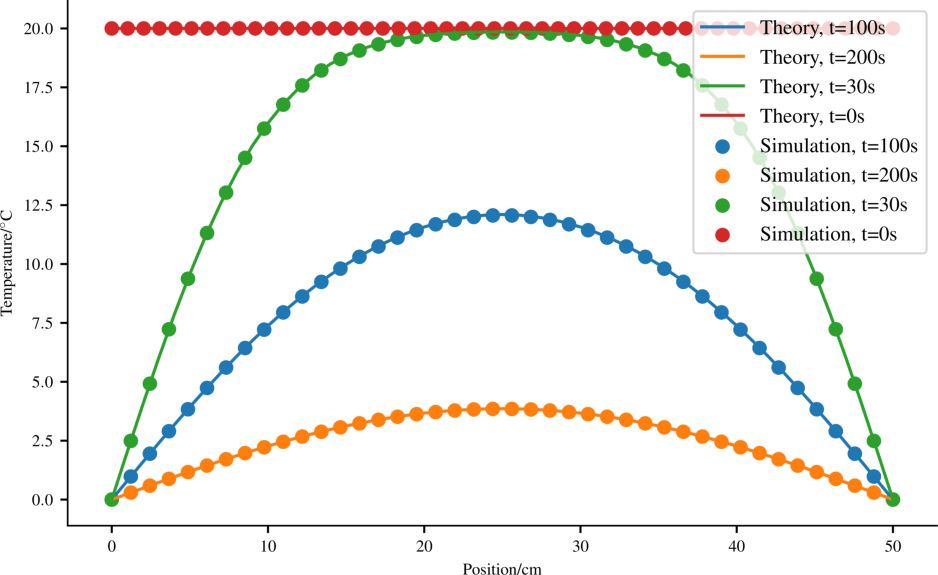
\includegraphics[width=.7\textwidth]{validation.pdf}
	\caption{Temperature profiles of the cube for various times, comparing between analytical solution and numerical method.}
	\label{fig:validation-heat}
\end{figure}	

\subsubsection*{MCRT and heat transport validation}


As a first test of the code, both \gls*{mcrt} and heat simulation, is compared to a simple analytical model of ablation. The simple model of ablation is as: the ablation energy ($E_a$), is defined as the minimum energy required to raise the temperature of the medium to 100~$^{\circ}$C, and then boil off the water in a volume dV, mass M. Thus, in one dimension~\cref{eqn:ablationenergy}, where the symbols have their usual meanings. If the energy for ablation is delivered in a time \textit{dt} by a laser of intensity ($Wcm^{-2}$), P, this gives \cref{eqn:midequationablation}.~\Cref{eqn:midequationablation} can be rearranged to give an ablation front velocity, \cref{eqn:ablationvelo}.


\begin{align}
E_a &= c_p \rho dx \Delta T + L_v \rho dx \label{eqn:ablationenergy}\\
P\cdot dt &= \rho dx (c_p \Delta T + L_v) \label{eqn:midequationablation} \\
u &= \frac{P}{\rho(c_p\Delta T+ L_v)} \label{eqn:ablationvelo}
\end{align}

Assuming the ablation front moves with constant velocity during the ablation, and using $L_v=2.53\cdot 10^6\ J kg^{-1},\ c_p=4181\ J\cdot kg^{-1}\cdot K^{-1}$ and the medium is a cube side $2\ mm$, with a starting temperature is 37~$^{\circ}$C with a water content of 70\% giving a density of 700~$kg\cdot m^{-3}$. For these parameters this gives an ablation velocity, $u\simeq 0.77\ cm\cdot s^{-1}$, and a time to ablate through 2~$mm$ of tissue of $\simeq 0.26~s$.
As the code developed in this chapter simulates the diffusion of heat in a medium due to an incident laser, the expected time to ablate through the same medium should be slightly larger as heat diffuses away from the voxel while it is being heated. When the full heat + \gls*{mcrt} code is used to simulate this experiment, it gives a time, $t \simeq 0.33~s$.	

%\medskip

%***maybe more? Could compare to https://doi.org/10.1117/1.2204615. They use MCRT + FDM but no ablation. So would be good test. Leaving till 2019 if time***


\section{\textit{In silco} results} 

\subsection{Introduction}

To match the experimental results,  an accurate model of the experimental setup \textit{in silico} must be created. However, due to computational constraints, such as memory and time available, some approximations to the experimental set-up have to be made. The porcine skin was a large thin slice of the top most layers of the skin. However, as the area of interest is where the ablation occurs, initially the porcine skin is modelled as a cuboid, dimensions:  1.1 $\times$ 1.1 $\times$ 0.5 cm. The initial temperature of the porcine skin is assumed to be around 5$^{\circ}$, as the tissue was kept on ice or was kept cooled. 
As mentioned in the previous sections, there are several unknowns in the model: \gls*{ta}, water content, temperature of air after ablation, and the exact thermal and optical properties of the porcine tissue. Therefore several models are run so that the full parameter space of these unknowns can be explored.
Results from these \textit{in silico} experiments are presented in this section along with a comparison of the model to the experimental work carried out in collaboration with the University of Dundee and the Photobiology department at Ninewells Hospital.


\subsubsection*{Optical \& thermal properties}
\label{sec:opticalprops}
The thermal and optical properties of porcine tissue are not known exactly for any given tissue sample. As such the thermal and optical properties used in this section are taken from various literature sources.

The laser used in the experimental work is an CO$_2$ laser operating at $10.6\ \mu m$. This means that the optical properties of the tissue are dominated by water absorption. The laser used in the experiment is the Pixel CO$_2$\cite{pixelco2}. The Pixel CO$_2$ laser has a wavelength 10.6$~\mu m$ which corresponds to an absorption coefficient in water of $\sim 850~cm^{-1}$. As the absorption coefficient is large, it is assumed that scattering is negligible at these wavelengths.
\Cref{table:values} summarises the thermal properties for tissue and air used in the simulations.  

% \begin{figure}	
% 	\centering
% 	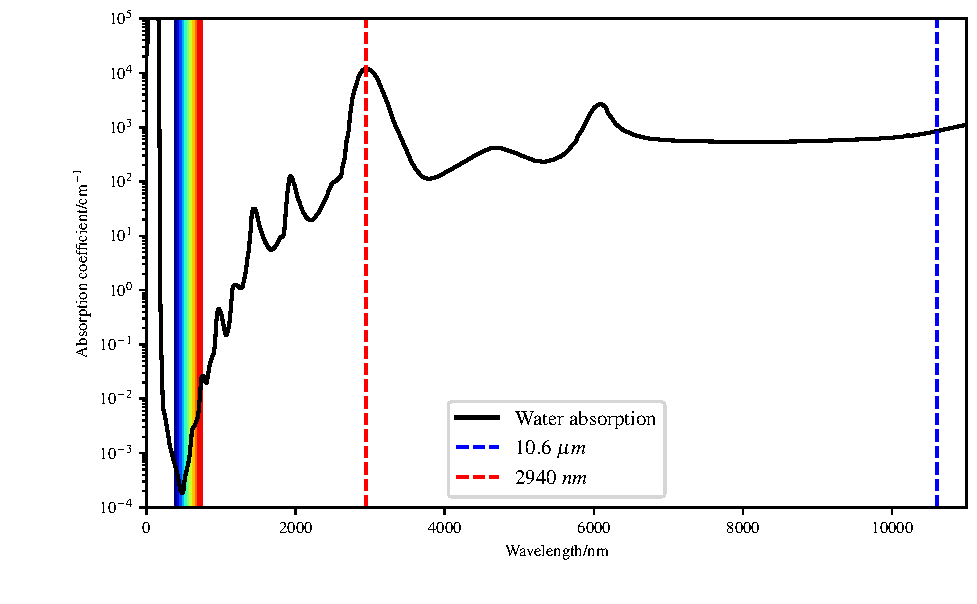
\includegraphics[width=.95\textwidth]{water.pdf}
% 	\caption{Water absorption coefficient for wavelengths 0-12000nm \cite{segelstein1981complex}. Data shows that water is highly absorbing in the infra-red portion of the spectrum  compared to the visible portion.}
% 	\label{fig:waterabsor}
% \end{figure}


The laser was used in ``Pixel beam'' mode. This means that the laser beam is split into an array of smaller beams. The laser used an array $9 \times 9$ of 81 pixel beams, each with a diameter of $250\ \mu m$. The Pixel CO$_2$ rated laser power is $\sim$ 70~$W$.

The laser delivered one single pulse of varying total energy delivered over the range 50~$mJ$ to 400~$mJ$, in so called ``super pulsed mode''. The experiment consisted of ablating the porcine tissue, as a function of energy per ``pixel'' beam. This was achieved by adjusting the pulse length of the laser, $\tau$, so that the energy per pulse was varied over a range 50~$mJ$ to 400~$mJ$.

\begin{table}
\begin{tabular}{|c|c|c|c|}
\hline 
• & Thermal conductivity, $\kappa$  & Density, $\rho$ & Heat capacity, c \\ 
\hline 
Tissue & $\rho \cdot (6.28\cdot 10^{-4}\cdot W + 1.17\cdot 10^{-4} \cdot P)$ & $\frac{1000}{W + 0.649\cdot P}$ & $4.2\cdot 10^{3}\cdot W + 1.09\cdot 10^{3}\cdot P$  \\ 
\hline 
Air & $a e^{-b(T-273.15)} +c$  & $\tfrac{p_{atm}}{R_{spec} T}$ & 1006 \\ 
\hline 
\end{tabular}
\caption{Optical and thermal properties for porcine tissue and air. W and P are the percentage of water and protein respectively. $\rho$ is the density of the skin, $p_{atm}$ is the pressure of air at 1 atmosphere, and $R_{spec}$ is the gas constant. $a$, $b$, and c are constants.}
\label{table:values}
\end{table}  

\subsubsection*{Computational speed up:}
As discussed in the~\cref{sec:intro}, the volume of interest is the area around the ablation craters. The volume is 1.1~$cm$ $\times$ 1.1~$cm$ $\times$ 0.5~$cm$. However, for the simulation to have good resolution of the ablation craters this volume would require many voxels for the tissue model. This is unfeasible due to: the memory required to store the various counters, grids, and variables, and the time that would be required to carry out the computation. Thus, the volume of interest is reduced to focus on just one of the ablation craters that is created by the laser (a volume of  0.06~$cm$ $\times$ 0.06~$cm$ $\times$ 0.18~$cm$) 
As a check to ensure that no physical phenomena are omitted by focusing on just one ablation crater, an initial simulation that models the full volume of interest was carried out to investigate the possibility of overlapping craters or other related phenomena. The simulation, as shown in~\cref{fig:sizecheck}, gives reassurance that the shrinking of the volume of interest is a valid approximation to make as there is no overlap between the separate ablation crater.
\begin{figure}[!htbp]
	\centering
    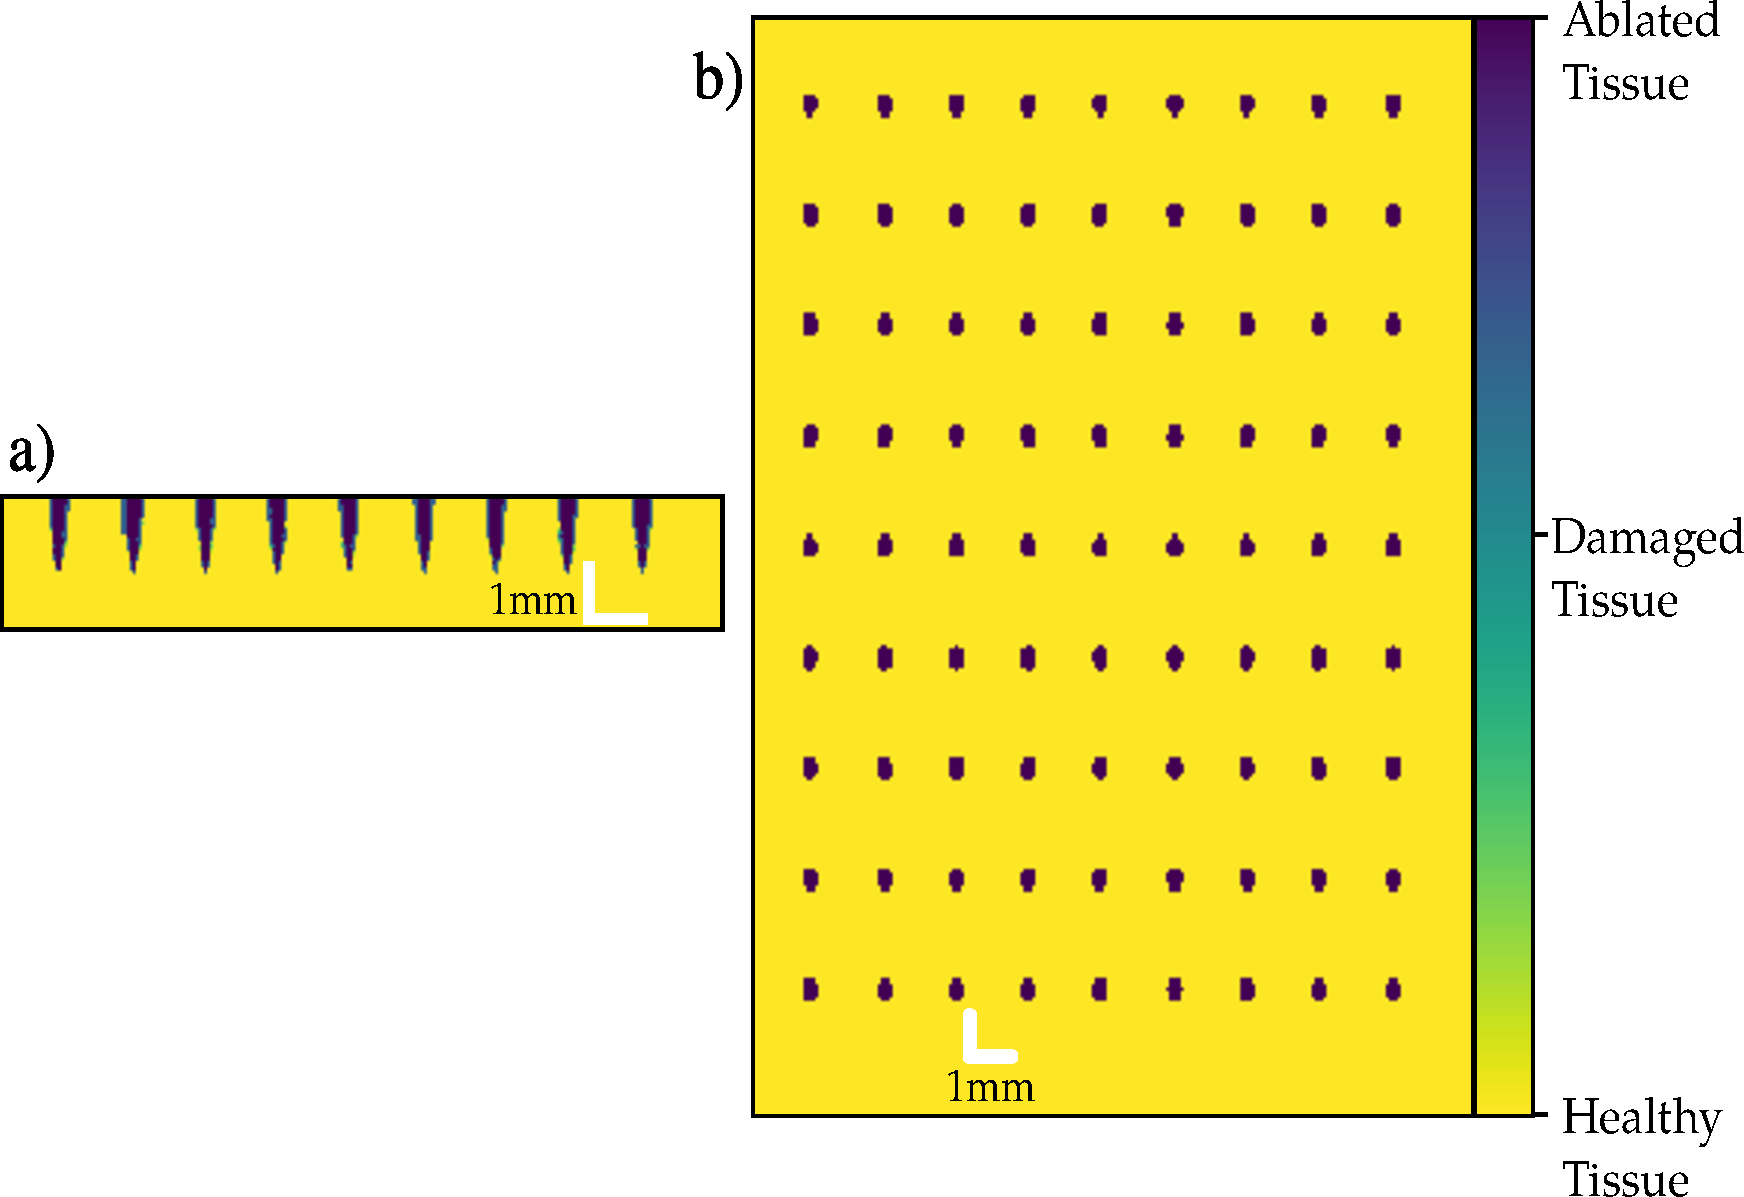
\includegraphics[width=.5\textwidth]{slice-poster.pdf}
    \caption{Simulation of 81 pixel beams. Figure a) shows a slice through the optical properties at the end of the simulation in the z-y plane. Figure b) shows the optical properties in the x-y plane at the top surface. Yellow is unchanged tissue, and purple is completely ablated tissue. Figure shows that the ablation craters do not overlap one another.}
    \label{fig:sizecheck}
\end{figure}


\subsection{Results}

\subsubsection*{Investigating ablation temperature, \texorpdfstring{$T_a$}{Ta}}

Various literature sources report the ablation temperature ranging widely from 177$^{\circ}$ to 500$^{\circ}$~\cite{gerstmann1994char,mckenzie1986three,sagi1992heating}. Thus, several models are run over this range to establish the \gls*{ta} which fits the experimental results. \Cref{fig:tacirc,fig:tagauss} show how \gls*{ta}, and beam profile affect the crater depth as a function of pixel beam energy for the CO$_2$ laser. The data suggests that a \gls*{ta} around $T_a=500~^{\circ}C$ is appropriate for the studies carried out, the upper limit of \gls*{ta} from the literature.

Increasing the ablation temperature has the obvious effect of requiring more energy to be deposited by the laser before ablation takes place. This also allows more heat to diffuse away from the ablation crater increasing the thermal damage to the surrounding tissue. Decreasing the ablation temperature has the converse effect, and allows the ablation crater to become deeper.

Over the full range of \gls*{ta}, as the energy per pixel beam increases, there is a trend that at higher energies the crater depth begins to taper off. This is potentially due to several reasons. As the ablation craters grows the volume of tissue that is ablated is replaced with air, allowing more heat loss from the tissue to the environment. As well as heat loss to the environment, more heat is diffused away into the surrounding tissue as the crater grows, due to the availability of more tissue for the heat to diffuse into.


\begin{figure}[!htbp]
	\centering
    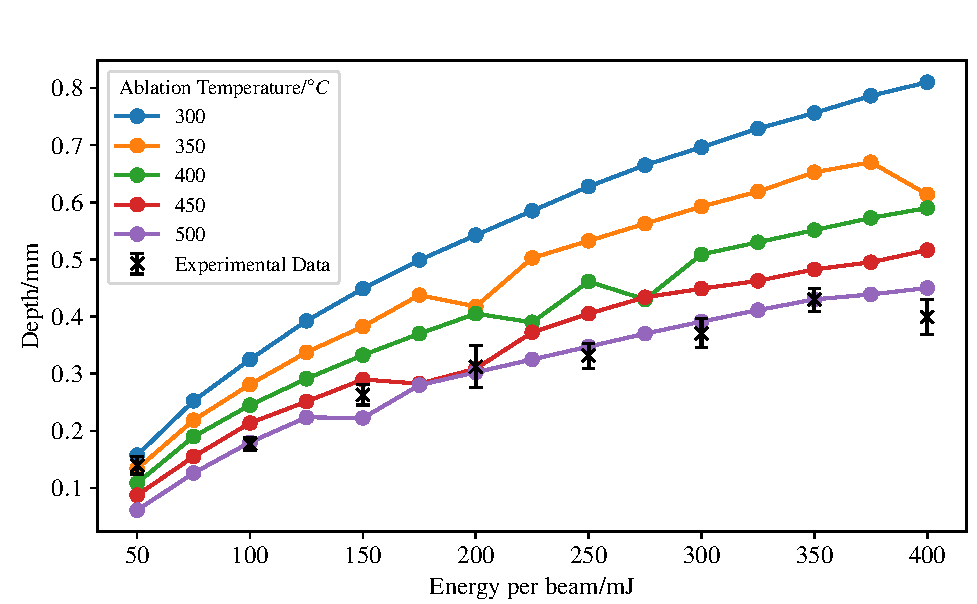
\includegraphics[width=.7\textwidth]{70w-circular.pdf}
    \caption{Simulation of 70~$W$ CO$_2$ ablative laser, with a circular beam profile. Crater depths as a function of pixel beam energy for various \gls*{ta}'s.}
    \label{fig:tacirc}
\end{figure}
 


\subsubsection*{Investigating beam type}

As the manufacturer does not provide information on the beam profile of the pixel beams and the lack of equipment available to measure the beam profile, the shape of the beam profile has to be assumed. Two different beam types are tried: Gaussian and circular (top-hat). \Cref{fig:tagauss,fig:tacirc} show the result of these \textit{in-silico} experiments. The Gaussian beam ablates deeper holes than the circular beam type, which is to be expected due to the distribution of power in the Gaussian beam. The beam that best fits the data is the circular beam. For the Gaussian beam to fit the data ablation would have to take place at temperatures above $500~^{\circ}C$ which does not fit with the literature. Without knowing the exact profile of the beam, it is assumed for the rest of the \textit{in-silico} experiments that the beam profile is circular.

 \begin{figure}[!htbp]
	\centering
    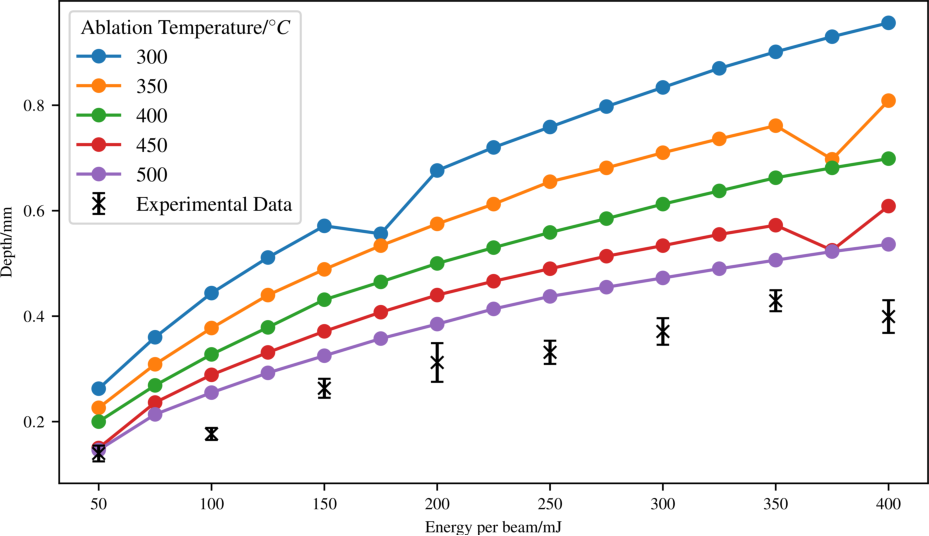
\includegraphics[width=.7\textwidth]{70w-gaussian.pdf}
    \caption{Simulation of 70~$W$ CO$_2$ ablative laser, with a Gaussian beam profile. Crater depths as a function of pixel beam energy for various \gls*{ta}'s.}
    \label{fig:tagauss}
\end{figure}

\subsubsection*{Temperature during ablation}

\Cref{fig:temp-500profile} shows slices of temperature as a function of time during a simulation for $T_a=500~^{\circ}C$.
This means that every column of pixels shows a bore hole through the medium (along the z axis) for a given time.
\Cref{fig:temp-500profile} also shows the laser pulse profile as a function of time as a reference so that knowledge of when the laser is on or off is easily elucidated.
The figure shows that the temperature reaches a maximum temperature which is equal to $T_a$, regardless of ablation progress.
This maximum temperature is researched roughly 0.25~s into the simulation, and lasts until $\sim$0.75~s.
The maximum temperature reaches a depth of around 0.04~cm into the tissue.
The region where water is boiling can be seen by the evidence of the ``dark valley'' before the abrupt jump in temperature to the maximum temperature.
\begin{figure}[!htbp]
	\centering
	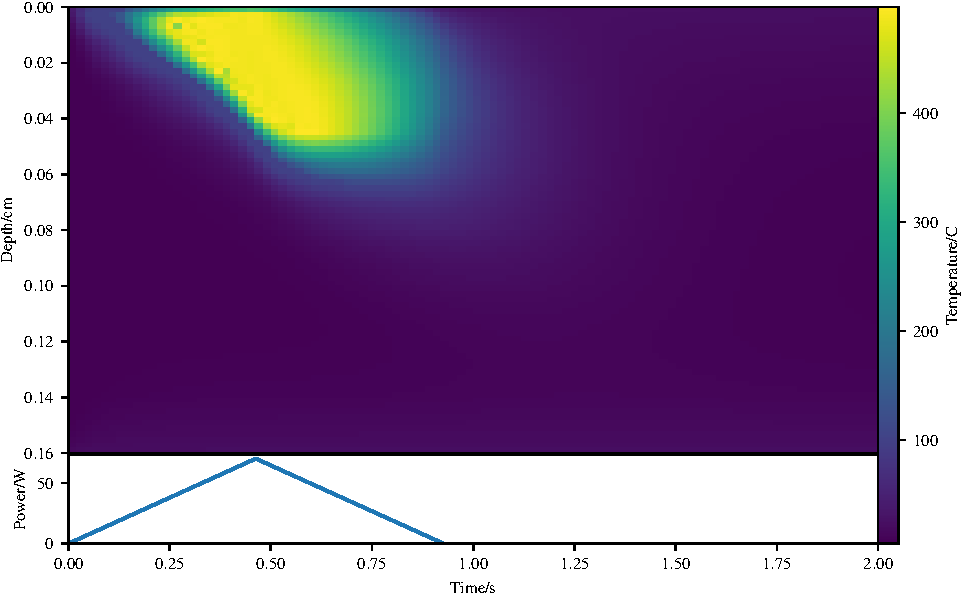
\includegraphics[width=0.7\textwidth]{temp-profile-middle.pdf}
	\caption{Temperature bore hole through centre of medium as a function of time, for~\gls*{ta}=500$~^{\circ}C$. Laser power is also plotted for comparison.}
	\label{fig:temp-500profile}
\end{figure}

The cause of this dark valley is due to the water in the tissue acting as a heat sink.
The water needs a large amount of energy to boil off, thus it stops the temperature from increasing until it boils off, giving rise to this dark valley.
This temperature maximum extends for a small distance into the tissue, before diffusion spreads it out.
Once the tissue ablates the ablated volume cools over the period of around 0.5~s.
Ablation continues until around 0.6~s, where the laser power has past its maximum value and no more ablation occurs.

\subsubsection*{Investigating thermal damage} 

As stated in~\cref{sec:coagdamage}, the Arrhenius damage integral is used to estimate the thermal damage due to the laser. To calculate the tissue damage around the ablation craters,~\cref{eqn:arrhenius} is first transformed into a summation:

\begin{align}
\Omega(t) &= \int^{t_{f}}_{t_p} Ae^{(-\tfrac{\Delta E}{RT})}d\tau \\
\Omega(t) &= \sum_{m=m_p}^{m_f} Ae^{(-\tfrac{\Delta E}{RT_{\xi}^{m}})}\Delta t\label{eqn:damagesum}
\end{align}
 
\noindent Where: 
	
	\indent $\Delta E$, $R$, $T$, and $A$ have the same meanings as before;
	
	\indent $\xi$ is the $i^{th}, j^{th}, k^{th}$ node;
	
	\indent and $m_p$ is the $p^{th}$ timestep when the $\xi^{th}$ node is above the threshold temperature.

	\medskip
	
	Using~\cref{eqn:damagesum} it can thus be estimated that the damage to the tissue on a voxel by voxel basis.~\Cref{fig:damfig} shows how far the thermal damage extends around the ablation crater. For ease of visualisation 1-3 is mapped to their respective burns via the following scheme, with $\eta$ as burn severity:
	
\begin{equation}
\eta = 
     \begin{cases}
       \text{3,} &\quad \Omega \geq 10000\\
       \text{2,} &\quad 1 \leq \Omega < 10000\\
       \text{1,} &\quad 0.53 \leq \Omega < 1\\
       \text{0,} &\quad 0.0 \leq \Omega< 0.53.\\
     \end{cases}
\label{eqn:thermalbound}
\end{equation}

\begin{figure}[!htbp]
	\centering
	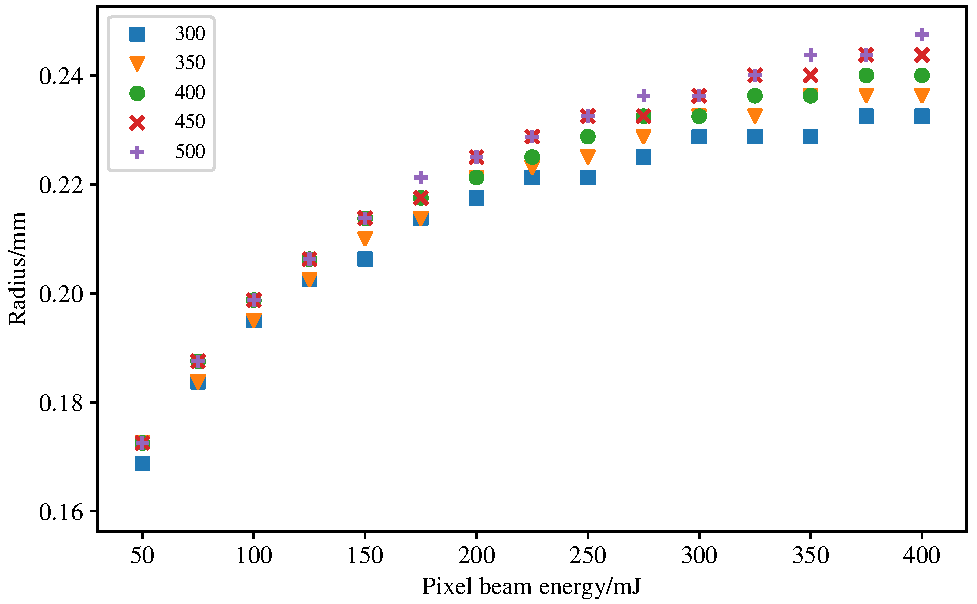
\includegraphics[width=0.7\textwidth]{horz-damage.pdf}
	\caption{Figure shows the maximum horizontal extent of thermal damage as a function of energy per pixel beam, for different $T_a$'s.}
	\label{fig:horz-70}
\end{figure}
	
As shown in~\cref{fig:damfig}, the thermal damage zone extends for a small distance around the ablation crater, due to the diffusion of heat into these areas. \Cref{fig:horz-70} shows the maximum horizontal thermal damage distance as a function of $T_a$, and pixel beam energy. For values of $T_a$ less than $\sim 425~^{\circ}C$, it appears that the maximum horizontal extent of the thermal damage begins to taper off. This is most likely because for lower values of $T_a$, there is a larger ablation crater, meaning that the energy from the laser is deposited deeper in the tissue in comparison to higher values of $T_a$. The higher values of $T_a$ allow greater diffusion of the heat, thus yielding larger zones of damage. Overall there is little difference in the maximum horizontal extent of thermal injury, when using different energies (of the order of $\sim$ 0.01~mm).



\begin{figure}[!htbp]
	\centering
	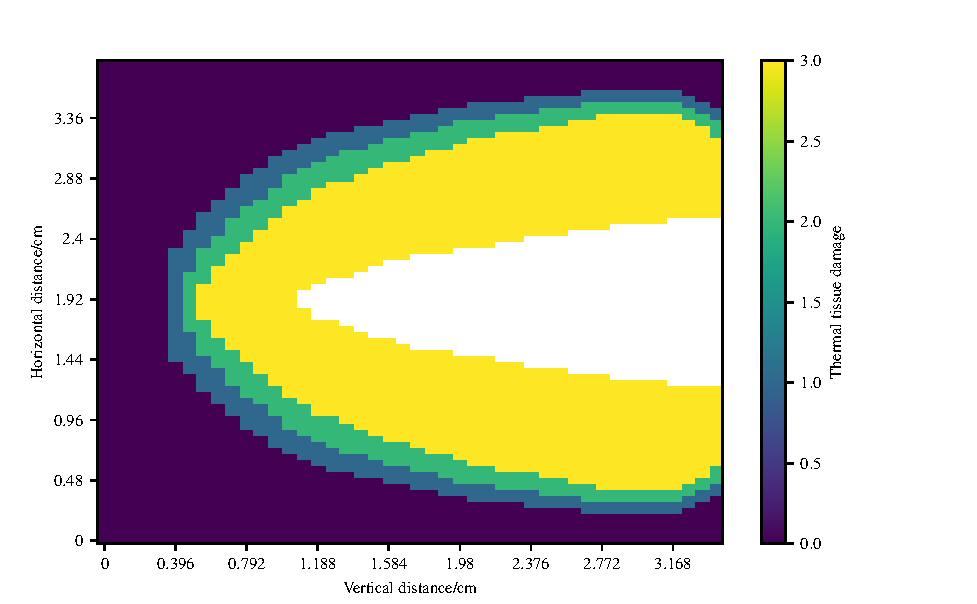
\includegraphics[width=.7\textwidth]{damage-slice.pdf}
	\caption{Tissue thermal damage around the ablation crater (white). Thermal tissue damage values of 3 refer to $3^{rd}$ degree burns, 2 to $2^{nd}$, and 1 to $1^{st}$ degree burns respectively. P is the power in Watts, $T_a$ is the ablation temperature in Kelvin, and $E_p$ is the energy per pixel beam in $mJ$.}
	\label{fig:damfig}
\end{figure}

Investigations for the time it takes for different areas of the tissue to become thermally damaged, were also carried out. This can be easily achieved by saving the time each voxel passes one of the damage boundaries in~\cref{eqn:thermalbound}.~\Cref{fig:time-thres1,fig:time-thres2} show the minimum time taken for $1^{st}$, $2^{nd}$, and $3^{rd}$ degree burns to occur as a function of depth. \Cref{fig:time-thres1} shows that there is little to no time (upon the order of $0.5$~$ms$) between $1^{st}$ and $2^{nd}$, and $3^{rd}$ degree burns.
\Cref{fig:time-thres2} shows there is a slightly greater time difference between $1^{st}$ and $2^{nd}$, and $3^{rd}$ degree burns, however this is almost as negligible as the 400~mJ case.

The reason that there is almost no time between $1^{st}$ and $2^{nd}$, and $3^{rd}$ degree burns, is most likely because there is little time for heat to diffuse, whilst the laser is still illuminating the medium. The laser pulses are on the order of seconds, and tissue is not thermally conductive. This leads to the results presented here.


\begin{figure}[!htbp]
	\squeezeup{2.5}
	\centering
	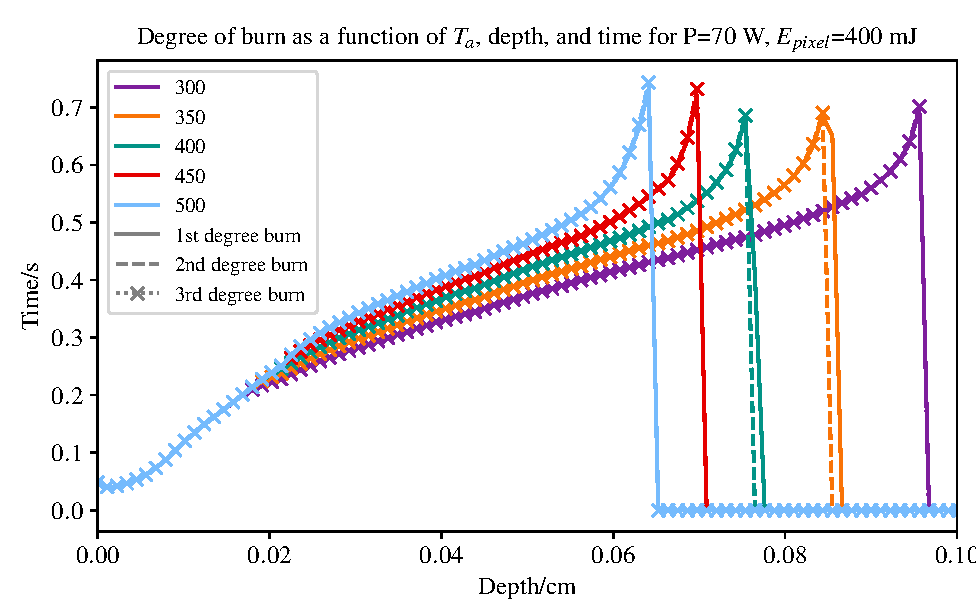
\includegraphics[width=0.7\textwidth]{70w-400.pdf}
	\caption{Figure shows the time taken for $1^{st},\ 2^{nd}$,and $3^{rd}$ to occur as a function of depth, for a range of $T_a$'s at 400~mJ.}
	\label{fig:time-thres1}
	\squeezeup{2.5}
\end{figure}	
	\FloatBarrier

\begin{figure}[!htbp]
	\squeezeup{2.5}

	\centering
	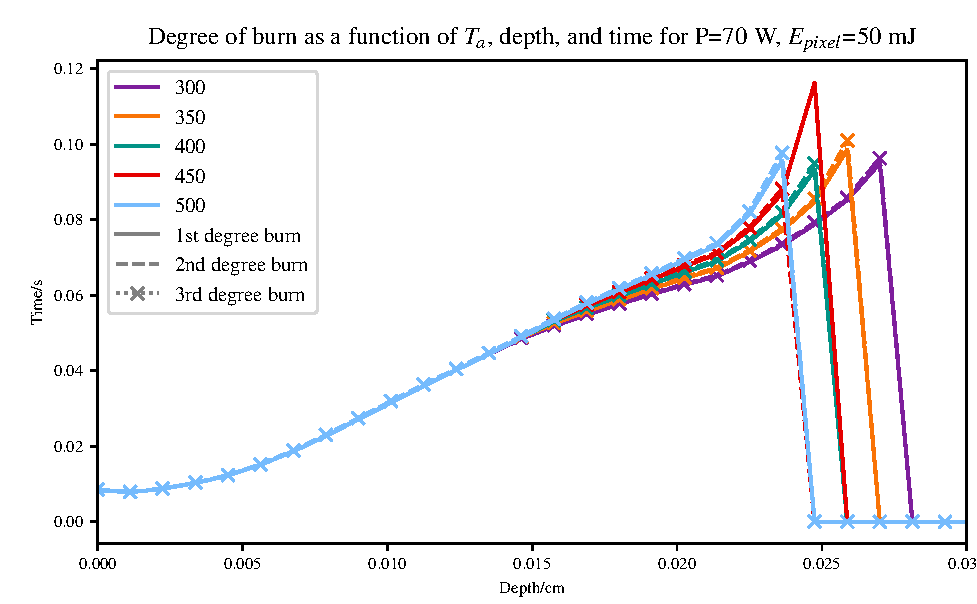
\includegraphics[width=0.7\textwidth]{70w-50.pdf}
	\caption{Figure shows the time taken for $1^{st},\ 2^{nd}$,and $3^{rd}$ to occur as a function of depth, for a range of $T_a$'s at 50~mJ.}
	\label{fig:time-thres2}
	\squeezeup{2.5}
\end{figure}	
\subsubsection*{Investigating laser pulse profile}

Pulsed lasers have a variety of pulse profiles.
The pulse profiles are usually modelled as triangular, tophat, or Gaussian.
However, the pulse profiles in reality are normally less well defined, and rather the pulse profile is something in between these perfect models.

The laser used in the above experiments, the Pixel CO$_2$, states that is has a triangular pulse profile for the laser pulses.
Thus, in this section the effect of the laser pulse profile has on ablation and the surrounding thermal injury is investigated.

Three different laser pulses profiles are investigated: tophat, triangular, and a Gaussian profiles.
The Gaussian profile used has approximately the same area as the two other pulses.

\Cref{fig:pulseprofiles} show the pulse profiles for a pulselength of $0.2~s$.
From \cref{fig:comparepulsetypes} the tophat pulse profile causes the most ablation, where as the Gaussian pulse causes the least.
This can be explained by the fact that the Gaussian pulse delivers energy over a longer time span, thus letting heat diffuse away before it can ``build'' up and cause damage, and thus ablation.

\begin{figure}[!htbp]
	\squeezeup{2.5}
	\centering
	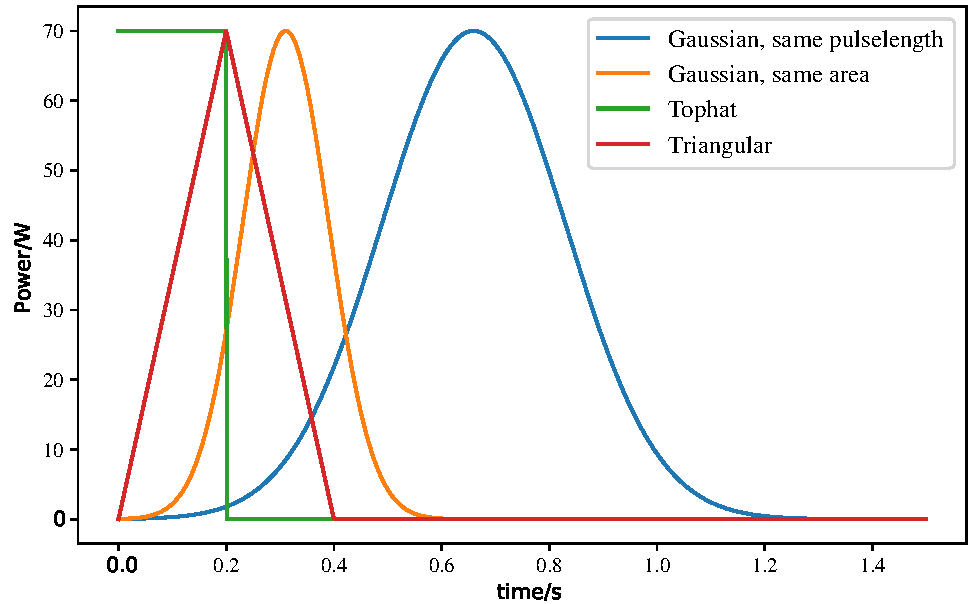
\includegraphics[width=0.6\textwidth]{profilespulse.pdf}
	\caption{Comparison of the different pulse profiles trialled for a pulselength of $0.2~s$.}
	\label{fig:pulseprofiles}
		\squeezeup{2.5}
\end{figure}

\begin{figure}[!htbp]
	\squeezeup{2.5}
	\centering
	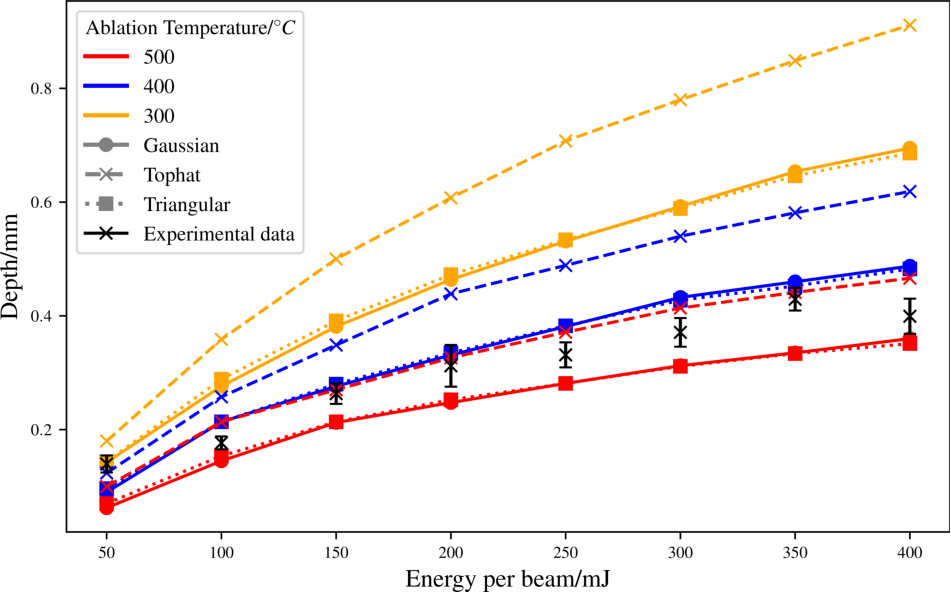
\includegraphics[width=0.6\textwidth]{pulsetypes-comp.pdf}
	\caption{Comparison of various pulse shapes for the pixel beams. Figure shows ablation depths for $T_a$=500$~^{\circ}C$.}
	\label{fig:comparepulsetypes}
		\squeezeup{2.5}
\end{figure}

\Cref{fig:pulsetypeburn} shows the difference between the pulse types with respect to the time it takes to reach a type of burn.
There is a large difference in profiles for each of the pulse types.
The Gaussian pulse type takes approximately 0.7~s to inflict a burn of any type.
Whereas the top hat pulse almost immediately inflict tissue damage, with the triangular pulse type takes approximately 0.05~s.
The profiles of the lines in~\cref{fig:pulsetypeburn} are also different when compared.
Both the Gaussian and triangular pulses have broadly the same shape, whereas the top hat beam has a gradual increasing curve.
This is due to the shape of the beams and their energy delivers per second.
The tophat beam delivers constant energy at $70~W$, where the other two beams peak output is $70~W$

\begin{figure}[!htbp]
	\squeezeup{2.5}
	\centering
	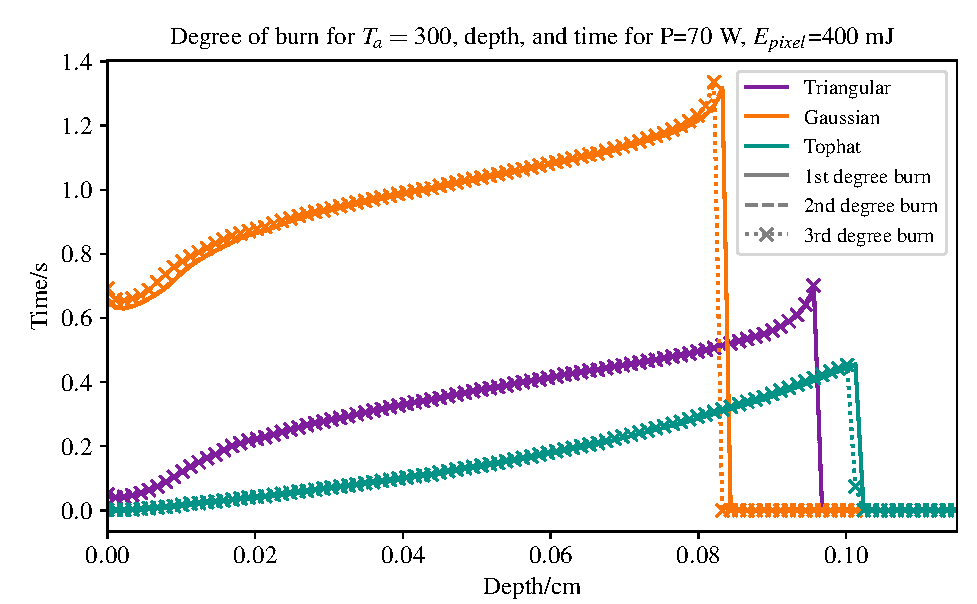
\includegraphics[width=0.6\textwidth]{time-burn-300-400.pdf}
	\caption{Figure shows a comparison of the time it takes to inflict a burn on tissue for laser with different pulse profiles.}
	\label{fig:pulsetypeburn}
	\squeezeup{2.5}
\end{figure}
\FloatBarrier
\subsubsection*{Investigating Initial Temperature}

As the experiment was carried out on porcine tissue that was kept on ice before the experiment was conducted, we assumed that the initial temperature of the porcine tissue was around 5$~^{\circ}C$.
This section investigates whether this is an accurate assumption.

To investigate this, three different temperatures were trialled: 0$~^{\circ}C$, 5$~^{\circ}C$, and 25$~^{\circ}C$.
These temperatures correspond to room temperature, the temperature of ice and the original temperature we assumed.
~\Cref{fig:pigtempcomp} shows the results of this \textit{in-silco} investigation.


\begin{figure}[!htbp]
	\centering
	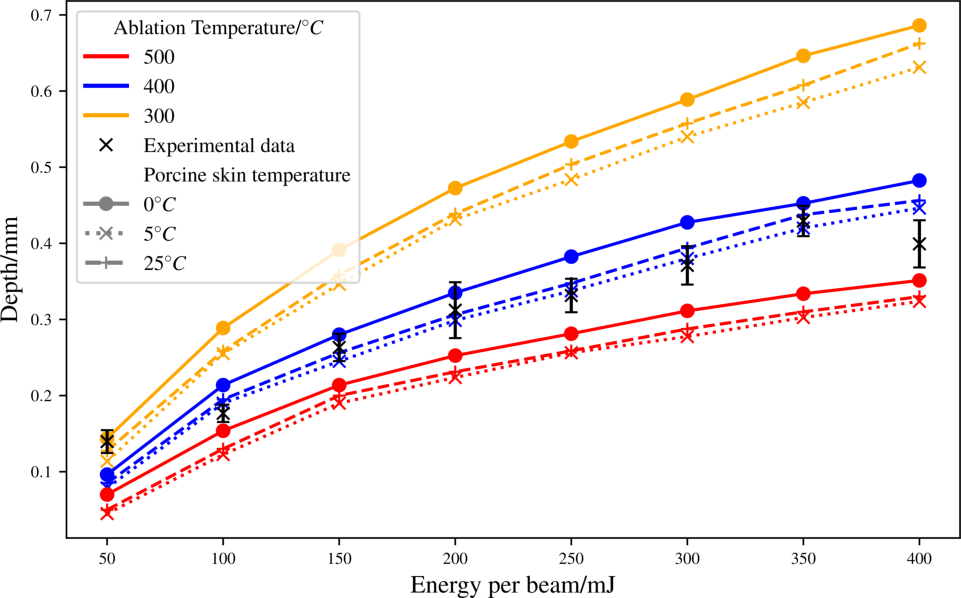
\includegraphics[width=0.7\textwidth]{pigtemps.pdf}
	\caption{Comparison of ablation depths for different initial temperatures in porcine skin.}
	\label{fig:pigtempcomp}
\end{figure}

As expected, the hotter the porcine skin is initially the larger the ablation depth.
This occurs as less energy is required to bring the porcine skin to its ablation temperature.
In the previous subsections it was assumed that the temperature of the porcine skin was around $5~^{\circ}C$.
This assumption was based upon the fact that the porcine skin was kept on ice before the experiment, thus the temperature of the skin must be between 0 and room temperature.
This investigation shows that over small variations of temperature ($\lessapprox 5~^{\circ}C$), the ablation depth does not vary too much (on the order of $\approx 0.01~mm$).

However, there is a greater difference in the maximum extent of thermal damage to the skin for different initial temperatures in porcine skin.
~\Cref{fig:horzdamagepig} shows this difference.


\begin{figure}[!htbp]
	\centering
	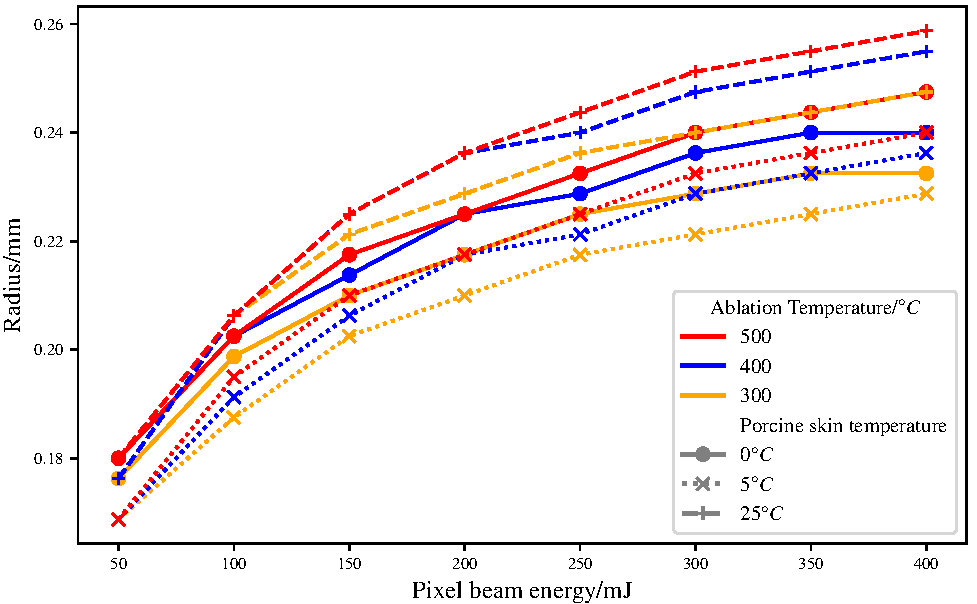
\includegraphics[width=0.7\textwidth]{Horz-damage-pigtemp.pdf}
	\caption{Comparison of maximum horizontal damage distance for different initial porcine skin temperatures.}
	\label{fig:horzdamagepig}
\end{figure}

\subsubsection*{Investigating Voxel Temperature After Ablation}

In the previous section it is assumed that the temperature of a voxel remains unchanged after the tissue is removed from that voxel via ablation.
However, this assumption may not be accurate as there should be some energy expended in the ablation process which would affect the temperature of the system.
To test to see how much this could affect the simulation, the temperature of the voxel after ablation was varied.
Two different temperatures were tried: half the ablation temperature and room temperature ($\approx 25~^{\circ}C$).
\Cref{fig:comparevoxtemp} shows the effect of the voxel temperature after ablation has on the ablation depth.

\begin{figure}[!htbp]
	\centering
	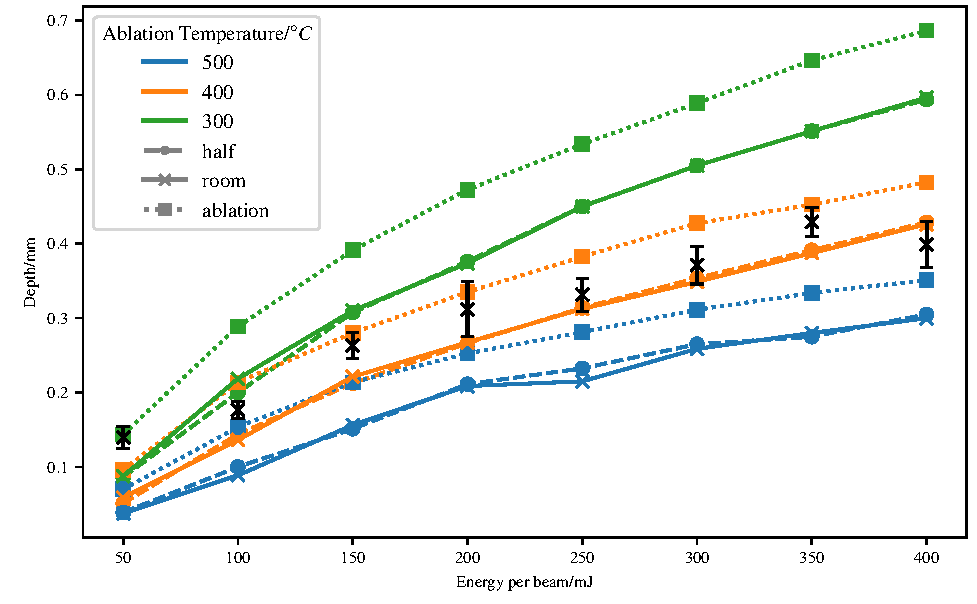
\includegraphics[width=0.7\textwidth]{compare-airtemp.pdf}
	\caption{Comparison of different voxel temperatures after ablation. Half refers to setting the temperature of a voxel to half that of the ablation temperature. Room refers to room temperature, and ablation leaves the temperature at the ablation temperature.}
	\label{fig:comparevoxtemp}
\end{figure}

Setting the voxel temperature to either half the ablation temperature or to room temperature has a large effect on the ablation depth, with a difference of $\approx 0.1~mm$.
However, there is a small difference between setting the voxel temperature to room temperature and to half of the ablation temperature though.

\section{Application of Model for Spy Disposal}

In the 1964 James Bond film Goldfinger, James Bond is threatened with a laser by the titular antagonist (see~\cref{fig:goldfinger}).
Would this laser actually cut Bond in half as the film implies, and could Goldfinger be more humane\footnote{i.e could Goldfinger use a laser that would lessen Bond's suffering.} in his choice of laser for the task?

As the first laser was demonstrated in 1960 was a ruby laser of $694~nm$, with the film being released in 1964 and the ``laser''\footnote{A laser was not used on set, but rather was added in post-production.} shown on screen being red, the likely laser portrayed is a ruby laser.

To assess whether Bond would die due to the laser we used the model outlined in this chapter with the following parameters.

As Auric Goldfinger uses this laser to cut sheets of gold, we assumed the power of the laser was around $1$~kW, as industrial lasers used to cut metal, are high powered continuous operation lasers.
We assumed that the Bond is completely made of skin, with no organs or bones.
We ran two simulations, one for the Ruby $694~nm$ and one for the $CO_2$ $10.6~\mu m$.
For the $CO_2$ as before there is no scattering due to high absorption coefficient. The Ruby laser's wavelength is highly scattering, so we model both scattering and absorption.
The medium we model is a $2~cm^3$ cube of homogeneous skin.

We found that the $CO_2$ takes $22~ms$, and Ruby takes $11~s$ to ablate through the $2~cm$ medium.
From timing the movie, the laser moves at a round $1~cms^{-1}$.
Therefore the Ruby laser used by Goldfinger would only give Bond some serious burns, but would leave him in one piece.
If Goldfinger used a $CO_2$ laser then Bond would have been cleanly cut in two.


\begin{figure}[!htpb]
	\centering
	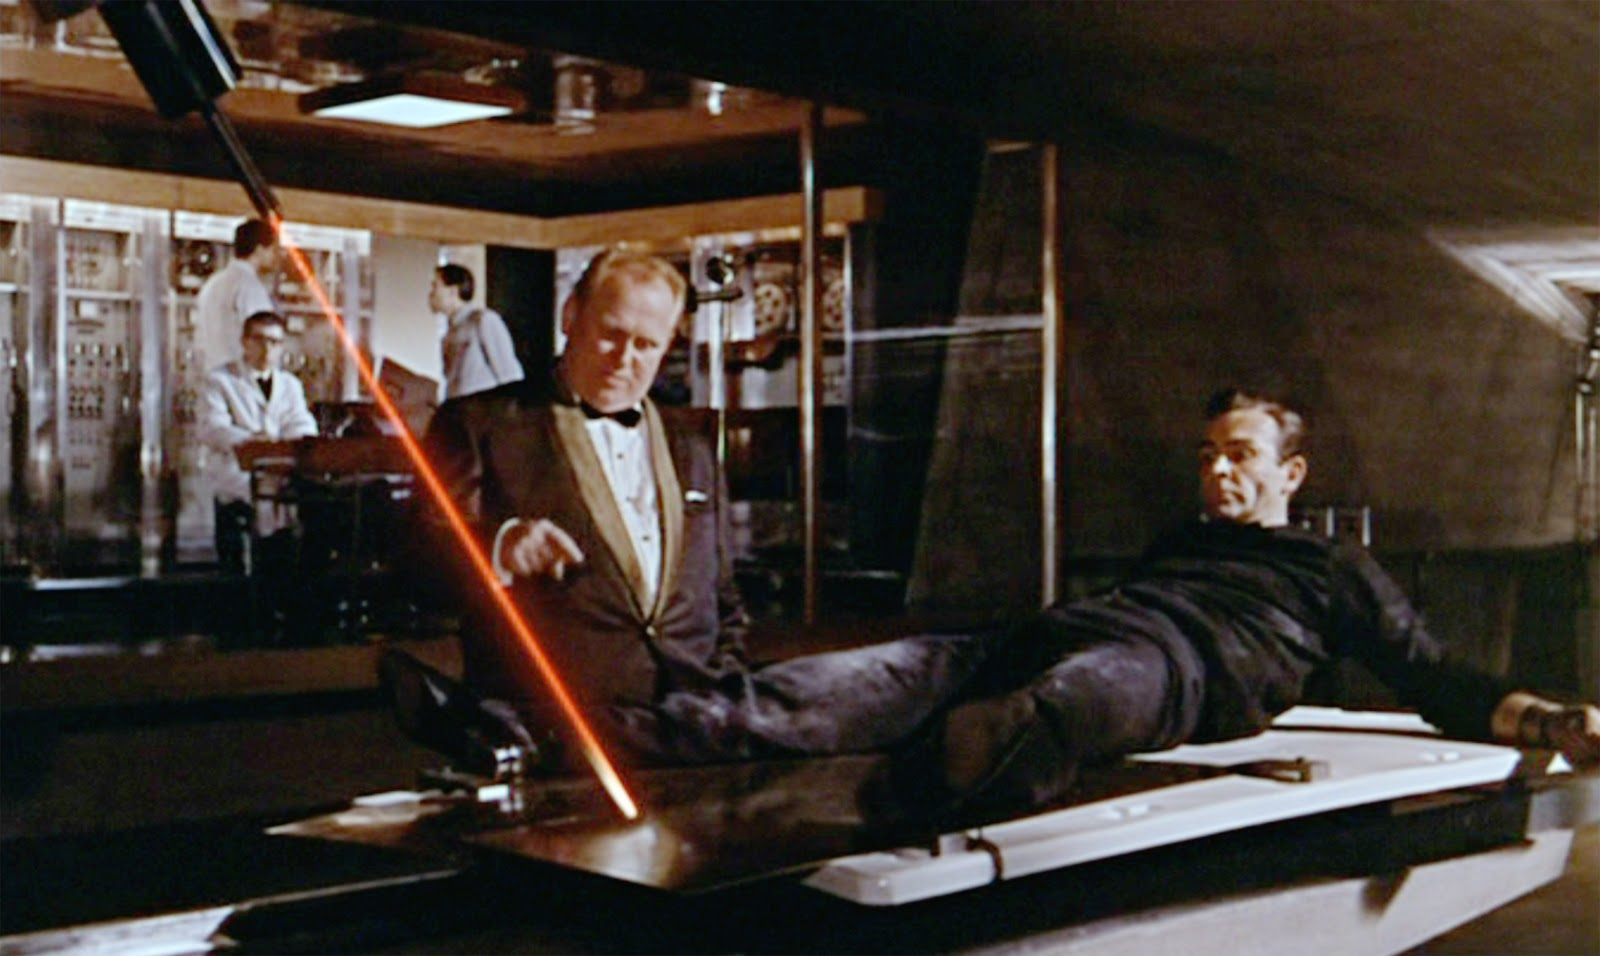
\includegraphics[width=0.5\textwidth]{goldfinger-laser.jpg}
	\caption{Still image of the iconic laser scene in the film Goldfinger. Copyrights Eon Productions.}
	\label{fig:goldfinger}
\end{figure}

\section{Conclusion}

Using \gls*{mcrt} and a finite difference method, a fully 3D model of photon and heat transport within tissue has been created. This model can be used to simulate the heat deposited by laser, the ablation craters formed via high powered lasers and the resultant thermal damage surrounding the ablation crater.

The model has been fully compared with both analytical solutions and experimental results. 
The model was found to match with experimental results that a tissue ablation temperature $T_a$ of around $500~^{\circ}C$ has to be adopted, toward the higher end of the range previously observed in the literature.

The simulations allow us to predict for a given laser power and pulse length, how much thermal damage is caused in the tissue, and how deep an ablation crater that will form. The computational model could be used in future to help develop treatment regimes for both aesthetic and medical procedures. For example, currently there is considerable amount of ``down time'' after skin rejuvenation, in which the patient displays inflammation, erythema, edema, pain, and crusting~\cite{lapidoth2014fractional,trelles2011safe,kohl2015fractional}. Simulations of thermal damage due to fractional ablation could help design treatment regimes that minimise these effects, whilst still delivering skin rejuvenation.
The model can also be applied to help optimise laser assisted drug delivery. 
Laser assisted drug delivery uses lasers to drill holes into the skin to help promote topical drug diffusion into the skin.
Our model can help predict the laser parameters needed to reach a certain hole depth, thus minimising thermal damage and pain to patients.

There are many avenues available with regards to future work on this model. The model presented here in this chapter was on an initially homogeneous skin model. In reality skin is composed of several distinct layers, with each layer containing varying amounts of different chromophores. Our model can easily incorporate an multi-layered skin model complete with various fractions of chromophores. However, as the laser used in these studies is an infra-red laser, water is the highest absorbing chromophore, meaning that a physically accurate model, with various chromophores is not need for this application.
The current model is a voxel based model, where all the voxels are the same size. This allows the model presented in this chapter to be easily set-up, with regards to parallelisation, optical/thermal properties and ease of programming. However, voxel models, where all the voxels are the same size, are not computationally efficient. Particularly in order to achieve good resolution, many voxels are needed, which requires large amounts of RAM, due to a $\sim n^3$ scaling of voxels to memory in 3D. A more efficient way, would be to allow different sizes of voxels, depending on parts of the model which need high resolution, and parts that do not need high resolution. Such a voxel model is called an \gls*{amr}. There are downsides to \gls*{amr}: complex implementation for parallelisation and set-up of optical/thermal properties, slower optical depth integration routines due to neighbour lookups.


